\documentclass[11pt]{article}

\usepackage[utf8]{inputenc}
\usepackage[T1]{fontenc}
\usepackage[french]{babel}
\usepackage{lmodern}
\usepackage[paperwidth=16cm,paperheight=9cm,margin=0cm]{geometry}
\usepackage{graphicx}
\usepackage{xcolor}
\usepackage{tikz}
\usetikzlibrary{calc,arrows.meta}
\usepackage[hidelinks]{hyperref}
\usepackage{multimedia}

\pagestyle{empty}
\setlength{\parindent}{0pt}
\pdfpageattr{/Group << /S /Transparency /I true /CS /DeviceRGB>>}

\definecolor{deepbrown}{HTML}{2B120B}
\definecolor{redbrown}{HTML}{5C1C12}
\definecolor{rust}{HTML}{B6401F}
\definecolor{orangehot}{HTML}{F47A1F}
\definecolor{amber}{HTML}{F4A322}
\definecolor{cream}{HTML}{FFF2DE}
\definecolor{softcream}{HTML}{F8D9B2}
\definecolor{teal}{HTML}{00A0A6}

\newcommand{\TutorRow}[5]{%
  \node[
    circle,
    minimum size=0.58cm,
    inner sep=0pt,
    draw=amber,
    line width=0.45pt,
    path picture={
      \node at (path picture bounding box.center)
        {\includegraphics[height=0.65cm]{#3}};
    }
  ] at ($(SW)+(#1,#2)$) {};
  \node[
    anchor=west,
    text=cream,
    font=\fontsize{5.6}{5.9}\selectfont\bfseries,
    text width=2.55cm,
    align=left
  ] at ($(SW)+(#1,#2)+(0.53,0.00)$) {#4};
}

\newcommand{\InitialRow}[5]{%
  \node[
    circle,
    minimum size=0.58cm,
    inner sep=0pt,
    draw=amber,
    line width=0.45pt,
    fill=rust,
    text=cream,
    font=\fontsize{5.2}{5.2}\selectfont\bfseries
  ] at ($(SW)+(#1,#2)$) {#3};
  \node[
    anchor=west,
    text=cream,
    font=\fontsize{5.6}{5.9}\selectfont\bfseries,
    text width=2.55cm,
    align=left
  ] at ($(SW)+(#1,#2)+(0.53,0.00)$) {#4};
}

\begin{document}

\begin{tikzpicture}[remember picture,overlay]
  \path (current page.south west) coordinate (SW);
  \path (current page.north east) coordinate (NE);

  \shade[left color=deepbrown,right color=redbrown] (SW) rectangle (NE);
  \fill[rust,opacity=0.42]
    (SW) -- ($(SW)+(6.2,0)$) -- ($(NE)+(-5.0,0)$) -- ($(NE)+(-9.8,0)$) -- cycle;
  \fill[orangehot,opacity=0.23]
    ($(SW)+(0,0)$) -- ($(SW)+(3.1,0)$) -- ($(NE)+(-7.1,0)$) -- ($(NE)+(-10.6,0)$) -- cycle;

  \node[anchor=center,opacity=0.25] at ($(SW)+(10.85,4.30)$)
    {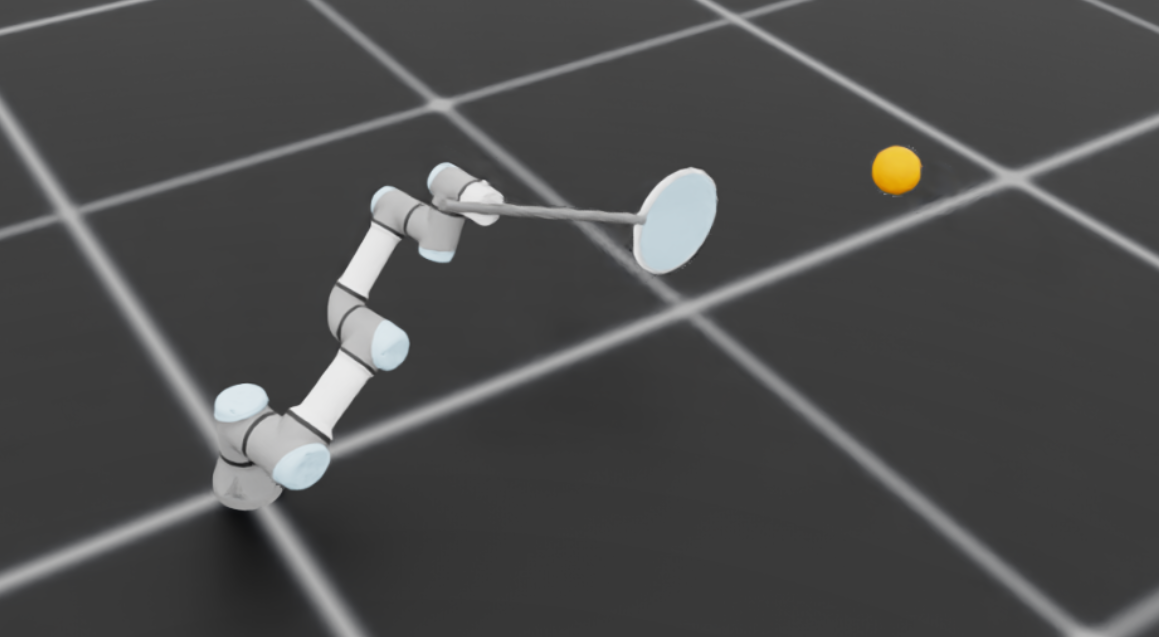
\includegraphics[width=8.9cm]{images/UR3e_Sim.png}};
  \fill[deepbrown,opacity=0.42] (SW) rectangle (NE);

  \draw[amber,opacity=0.80,line width=1.0pt]
    ($(SW)+(1.04,3.12)$) .. controls ($(SW)+(4.25,6.10)$) and ($(SW)+(8.35,6.15)$) .. ($(SW)+(12.45,4.18)$);
  \draw[orangehot,opacity=0.42,line width=4.4pt]
    ($(SW)+(1.00,3.10)$) .. controls ($(SW)+(4.20,6.05)$) and ($(SW)+(8.30,6.08)$) .. ($(SW)+(12.45,4.18)$);
  \shade[ball color=amber] ($(SW)+(12.65,4.28)$) circle (0.20cm);

  \fill[softcream!86!orangehot,opacity=0.96,rounded corners=3pt]
    ($(SW)+(0.34,8.58)$) rectangle ($(SW)+(10.46,7.62)$);
  \draw[orangehot,opacity=0.88,line width=0.45pt,rounded corners=3pt]
    ($(SW)+(0.34,8.58)$) rectangle ($(SW)+(10.46,7.62)$);

  \node[anchor=west,inner sep=0pt]
    at ($(SW)+(0.62,8.10)$)
    {
\includegraphics[height=0.58cm]{images/logos/Institut_pascal.png}};
  \node[anchor=west,inner sep=0pt]
    at ($(SW)+(2.20,8.10)$)
    {
\includegraphics[width=4.95cm]{images/logos/cir_itps.png}};
  \node[anchor=west,inner sep=0pt]
    at ($(SW)+(7.44,8.10)$)
    {
\includegraphics[width=2.95cm]{images/logos/isite_cap_20_25.png}};

  \node[
    anchor=west,
    text=cream,
    font=\fontsize{36}{38}\selectfont\bfseries
  ] at ($(SW)+(0.92,5.98)$) {Catch a ball};

  \draw[orangehot,line width=1.0pt]
    ($(SW)+(1.00,5.48)$) -- ($(SW)+(5.72,5.48)$);
  \draw[amber,line width=0.45pt,opacity=0.75]
    ($(SW)+(1.00,5.36)$) -- ($(SW)+(3.55,5.36)$);

  \node[
    anchor=west,
    text=cream,
    font=\fontsize{11}{12}\selectfont,
    text width=6.35cm,
    align=left
  ] at ($(SW)+(1.02,4.60)$)
    {Détection et estimation 3D d'une balle rapide par caméra événementielle};

  \node[
    anchor=west,
    text=softcream,
    font=\fontsize{7.5}{8.5}\selectfont,
    text width=6.2cm,
    align=left
  ] at ($(SW)+(1.03,3.70)$)
    {Stage M1 Mécatronique | Rigon Ajvazi | 2026};

  \fill[deepbrown,opacity=0.67,rounded corners=4pt]
    ($(SW)+(11.78,1.62)$) rectangle ($(SW)+(15.55,5.95)$);
  \draw[orangehot,opacity=0.82,line width=0.65pt,rounded corners=4pt]
    ($(SW)+(11.78,1.62)$) rectangle ($(SW)+(15.55,5.95)$);
  \node[
    anchor=north west,
    text=amber,
    font=\fontsize{6.7}{7.4}\selectfont\bfseries
  ] at ($(SW)+(12.02,5.70)$) {Encadrement};

  \TutorRow{12.40}{4.86}{images/Tuteurs/Sebastien_Lengagne.jpeg}{Sébastien\\Lengagne}{}
  \InitialRow{12.40}{4.06}{CT}{Céline\\Teulière}{}
  \TutorRow{12.40}{3.18}{images/Tuteurs/Antonio.jpeg}{Antonio Claudio\\de Sousa dos\\Santos Filho}{}
  \TutorRow{12.40}{2.16}{images/Tuteurs/Benoit_Thuilot.jpg}{Benoit\\Thuilot}{}

  \node[
    anchor=south east,
    text=softcream,
    font=\fontsize{4.7}{5.0}\selectfont,
    opacity=0.75
  ] at ($(SW)+(15.50,0.40)$) {1 / 13};
\end{tikzpicture}

\newpage

\begin{tikzpicture}[remember picture,overlay]
  \path (current page.south west) coordinate (SW);
  \path (current page.north east) coordinate (NE);

  \shade[left color=deepbrown,right color=redbrown] (SW) rectangle (NE);
  \fill[rust,opacity=0.36]
    (SW) -- ($(SW)+(5.8,0)$) -- ($(NE)+(-5.2,0)$) -- ($(NE)+(-9.4,0)$) -- cycle;
  \fill[orangehot,opacity=0.18]
    ($(SW)+(0,0)$) -- ($(SW)+(2.8,0)$) -- ($(NE)+(-7.5,0)$) -- ($(NE)+(-10.9,0)$) -- cycle;
  \fill[deepbrown,opacity=0.26] (SW) rectangle (NE);

  \node[
    anchor=west,
    text=cream,
    font=\fontsize{20}{22}\selectfont\bfseries
  ] at ($(SW)+(0.72,8.20)$) {Organisation d'accueil};
  \draw[orangehot,line width=0.85pt] ($(SW)+(0.74,7.88)$) -- ($(SW)+(5.40,7.88)$);
  \draw[amber,line width=0.40pt,opacity=0.75] ($(SW)+(0.74,7.75)$) -- ($(SW)+(3.25,7.75)$);

  \tikzset{
    panel/.style={
      fill=deepbrown,
      fill opacity=0.56,
      draw=orangehot,
      draw opacity=0.82,
      line width=0.55pt,
      rounded corners=5pt
    },
    orgmain/.style={
      fill=cream,
      fill opacity=0.95,
      draw=amber,
      line width=0.45pt,
      rounded corners=3pt,
      text=redbrown,
      align=center,
      font=\fontsize{6.5}{7.2}\selectfont\bfseries,
      minimum height=0.54cm
    },
    orgsub/.style={
      fill=redbrown,
      fill opacity=0.90,
      draw=orangehot,
      line width=0.35pt,
      rounded corners=3pt,
      text=cream,
      align=center,
      font=\fontsize{5.0}{5.6}\selectfont\bfseries,
      minimum height=0.36cm
    },
    chip/.style={
      fill=rust,
      fill opacity=0.86,
      draw=amber,
      line width=0.30pt,
      rounded corners=2.5pt,
      text=cream,
      align=center,
      font=\fontsize{4.8}{5.2}\selectfont,
      minimum height=0.40cm
    },
    link/.style={-{Latex[length=1.5mm]},draw=amber,opacity=0.86,line width=0.38pt}
  }

  \path[panel] ($(SW)+(0.62,0.74)$) rectangle ($(SW)+(7.68,7.36)$);
  \node[anchor=west,text=amber,font=\fontsize{7.0}{7.6}\selectfont\bfseries]
    at ($(SW)+(0.92,7.02)$) {Institut Pascal};
  \node[anchor=west,text=softcream,font=\fontsize{4.8}{5.2}\selectfont]
    at ($(SW)+(0.94,6.70)$) {UMR 6602};

  \node[orgmain,text width=2.08cm] (tutelles) at ($(SW)+(4.02,6.54)$) {Tutelles\\UCA / CNRS};
  \node[orgmain,text width=2.40cm] (ip) at ($(SW)+(4.02,5.58)$) {Institut Pascal\\sciences de l'ingénierie};
  \node[orgsub,text width=1.08cm] (gepeb) at ($(SW)+(1.20,4.76)$) {GePEB};
  \node[orgsub,text width=1.08cm] (ispr) at ($(SW)+(2.61,4.76)$) {ISPR};
  \node[orgsub,text width=1.08cm] (m3g) at ($(SW)+(4.02,4.76)$) {M3G};
  \node[orgsub,text width=1.08cm,font=\fontsize{4.5}{5.0}\selectfont\bfseries] (photon) at ($(SW)+(5.43,4.76)$) {PHOTON};
  \node[orgsub,text width=1.08cm] (tgi) at ($(SW)+(6.84,4.76)$) {TGI};
  \draw[link] (tutelles) -- (ip);
  \foreach \x in {gepeb,ispr,m3g,photon,tgi} { \draw[link] (ip) -- (\x); }

  \node[orgmain,text width=2.55cm] (maccs) at ($(SW)+(2.28,3.48)$) {MACCS\\robotique et commande};
  \node[orgmain,text width=2.55cm] (comsee) at ($(SW)+(5.50,3.48)$) {ComSee\\vision et perception};
  \draw[link] (ispr) -- (maccs);
  \draw[link] (ispr) -- (comsee);

  \node[circle,minimum size=0.55cm,inner sep=0pt,draw=amber,line width=0.4pt,
    path picture={\node at (path picture bounding box.center)
      {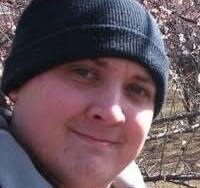
\includegraphics[height=0.63cm]{images/Tuteurs/Sebastien_Lengagne.jpeg}};}]
    at ($(SW)+(1.64,2.62)$) {};
  \node[anchor=north,text=cream,font=\fontsize{4.8}{5.1}\selectfont\bfseries,align=center]
    at ($(SW)+(1.64,2.24)$) {Sébastien\\Lengagne};
  \node[circle,minimum size=0.55cm,inner sep=0pt,draw=amber,line width=0.4pt,
    path picture={\node at (path picture bounding box.center)
      {
\includegraphics[height=0.63cm]{images/Tuteurs/Antonio.jpeg}};}]
    at ($(SW)+(2.88,2.62)$) {};
  \node[anchor=north,text=cream,font=\fontsize{4.6}{4.9}\selectfont\bfseries,align=center]
    at ($(SW)+(2.88,2.24)$) {Antonio\\C. de Sousa};

  \node[circle,minimum size=0.55cm,inner sep=0pt,draw=amber,line width=0.4pt,
    fill=rust,text=cream,font=\fontsize{5.0}{5.0}\selectfont\bfseries]
    at ($(SW)+(5.50,2.62)$) {CT};
  \node[anchor=north,text=cream,font=\fontsize{4.8}{5.1}\selectfont\bfseries,align=center]
    at ($(SW)+(5.50,2.24)$) {Céline\\Teulière};

  \fill[orangehot,opacity=0.16,rounded corners=3pt]
    ($(SW)+(3.98,0.82)$) rectangle ($(SW)+(7.42,1.58)$);
  \draw[amber,opacity=0.65,line width=0.25pt,rounded corners=3pt]
    ($(SW)+(3.98,0.82)$) rectangle ($(SW)+(7.42,1.58)$);
  \node[circle,minimum size=0.46cm,inner sep=0pt,draw=amber,line width=0.35pt,
    path picture={\node at (path picture bounding box.center)
      {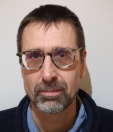
\includegraphics[height=0.53cm]{images/Tuteurs/Benoit_Thuilot.jpg}};}]
    at ($(SW)+(4.34,1.20)$) {};
  \node[anchor=west,text=cream,font=\fontsize{4.4}{4.7}\selectfont\bfseries,align=left,text width=0.92cm]
    at ($(SW)+(4.68,1.23)$) {Benoit\\Thuilot};
  \node[anchor=west,text=softcream,font=\fontsize{4.0}{4.3}\selectfont,align=left,text width=1.20cm]
    at ($(SW)+(6.02,1.23)$) {UCA /\\Inst. Pascal};

  \path[panel] ($(SW)+(8.18,0.74)$) rectangle ($(SW)+(15.38,7.36)$);
  \node[anchor=west,text=amber,font=\fontsize{7.0}{7.6}\selectfont\bfseries]
    at ($(SW)+(8.48,7.02)$) {CIR ITPS};
  \node[anchor=west,text=softcream,font=\fontsize{4.8}{5.2}\selectfont]
    at ($(SW)+(8.50,6.70)$) {transport + production};

  \node[orgmain,text width=2.16cm] (cap) at ($(SW)+(11.80,6.18)$) {CAP 20-25\\I-SITE};
  \node[orgmain,text width=2.56cm] (cir) at ($(SW)+(11.80,5.18)$) {CIR ITPS\\transports et production};
  \draw[link] (cap) -- (cir);

  \node[chip,text width=1.62cm] (res) at ($(SW)+(9.42,4.34)$) {Ressourcement};
  \node[chip,text width=1.62cm] (tai) at ($(SW)+(11.80,4.02)$) {Transports\\automatisés};
  \node[chip,text width=1.62cm] (uf) at ($(SW)+(14.12,4.34)$) {Usine\\du futur};
  \node[chip,text width=1.62cm] (agro) at ($(SW)+(9.42,3.12)$) {Agro-\\technologies};
  \node[chip,text width=1.62cm] (serv) at ($(SW)+(11.80,2.78)$) {Services\\innovants};
  \node[chip,text width=1.62cm] (ene) at ($(SW)+(14.12,3.12)$) {Énergies\\du futur};
  \node[chip,text width=1.62cm] (proto) at ($(SW)+(11.80,1.70)$) {Prototypage};
  \draw[link] (cir.south west) -- (res.east);
  \draw[link] (cir.south east) -- (uf.west);
  \draw[link] (cir.south west) -- (agro.north east);
  \draw[link] (cir.south east) -- (ene.north west);
  \draw[link] (cir.south) -- (tai.north);
  \draw[link] (tai.south) -- (serv.north);
  \draw[link] (serv.south) -- (proto.north);

  \fill[orangehot,opacity=0.18,rounded corners=3pt]
    ($(SW)+(8.62,1.06)$) rectangle ($(SW)+(14.96,1.50)$);
  \node[
    anchor=center,
    text=cream,
    font=\fontsize{5.0}{5.4}\selectfont\bfseries,
    text width=5.85cm,
    align=center
  ] at ($(SW)+(11.79,1.28)$) {Perception rapide + interception robotique};
  \node[
    anchor=south east,
    text=softcream,
    font=\fontsize{4.7}{5.0}\selectfont,
    opacity=0.75
  ] at ($(SW)+(15.50,0.40)$) {2 / 13};
\end{tikzpicture}

\newpage

\begin{tikzpicture}[remember picture,overlay]
  \path (current page.south west) coordinate (SW);
  \path (current page.north east) coordinate (NE);

  \shade[left color=deepbrown,right color=redbrown] (SW) rectangle (NE);
  \fill[rust,opacity=0.34]
    (SW) -- ($(SW)+(5.5,0)$) -- ($(NE)+(-5.4,0)$) -- ($(NE)+(-9.2,0)$) -- cycle;
  \fill[orangehot,opacity=0.18]
    ($(SW)+(0,0)$) -- ($(SW)+(2.5,0)$) -- ($(NE)+(-7.6,0)$) -- ($(NE)+(-10.8,0)$) -- cycle;
  \fill[deepbrown,opacity=0.25] (SW) rectangle (NE);

  \node[
    anchor=west,
    text=cream,
    font=\fontsize{20}{22}\selectfont\bfseries
  ] at ($(SW)+(0.72,8.20)$) {Plan général du projet};
  \draw[orangehot,line width=0.85pt] ($(SW)+(0.74,7.88)$) -- ($(SW)+(5.70,7.88)$);
  \draw[amber,line width=0.40pt,opacity=0.75] ($(SW)+(0.74,7.75)$) -- ($(SW)+(3.25,7.75)$);

  \tikzset{
    planpanel/.style={
      fill=deepbrown,
      fill opacity=0.58,
      draw=orangehot,
      draw opacity=0.84,
      line width=0.55pt,
      rounded corners=5pt
    },
    planarrow/.style={-{Latex[length=2.1mm]},draw=amber,opacity=0.92,line width=0.72pt},
    planlabel/.style={
      text=cream,
      font=\fontsize{8.4}{9.0}\selectfont\bfseries,
      align=center
    },
    plansub/.style={
      text=softcream,
      font=\fontsize{5.2}{5.7}\selectfont,
      align=center,
      text width=3.34cm
    }
  }

  \path[planpanel] ($(SW)+(0.72,1.12)$) rectangle ($(SW)+(4.84,7.14)$);
  \path[planpanel] ($(SW)+(5.94,1.12)$) rectangle ($(SW)+(10.06,7.14)$);
  \path[planpanel] ($(SW)+(11.16,1.12)$) rectangle ($(SW)+(15.28,7.14)$);

  \node[circle,fill=orangehot,draw=amber,line width=0.35pt,text=cream,
    font=\fontsize{7.2}{7.2}\selectfont\bfseries,minimum size=0.48cm]
    at ($(SW)+(1.18,6.68)$) {1};
  \node[planlabel,text width=2.86cm] at ($(SW)+(2.78,6.62)$) {Perception\\événementielle};
  \node[anchor=center,opacity=0.76] at ($(SW)+(2.78,4.42)$)
    {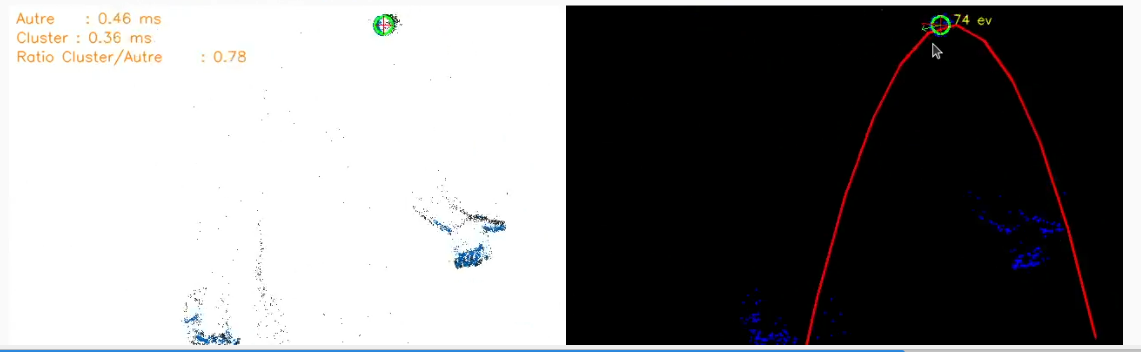
\includegraphics[width=3.72cm]{images/Algo_Cricle_Fitting/Sortie_algo_2D.png}};
  \node[plansub] at ($(SW)+(2.78,2.36)$)
    {calibration intrinsèque\\calibration extrinsèque\\position 3D};

  \node[circle,fill=orangehot,draw=amber,line width=0.35pt,text=cream,
    font=\fontsize{7.2}{7.2}\selectfont\bfseries,minimum size=0.48cm]
    at ($(SW)+(6.40,6.68)$) {2};
  \node[planlabel,text width=2.90cm] at ($(SW)+(8.00,6.62)$) {Simulation\\Isaac Sim / Lab};
  \node[anchor=center,opacity=0.72] at ($(SW)+(8.00,4.44)$)
    {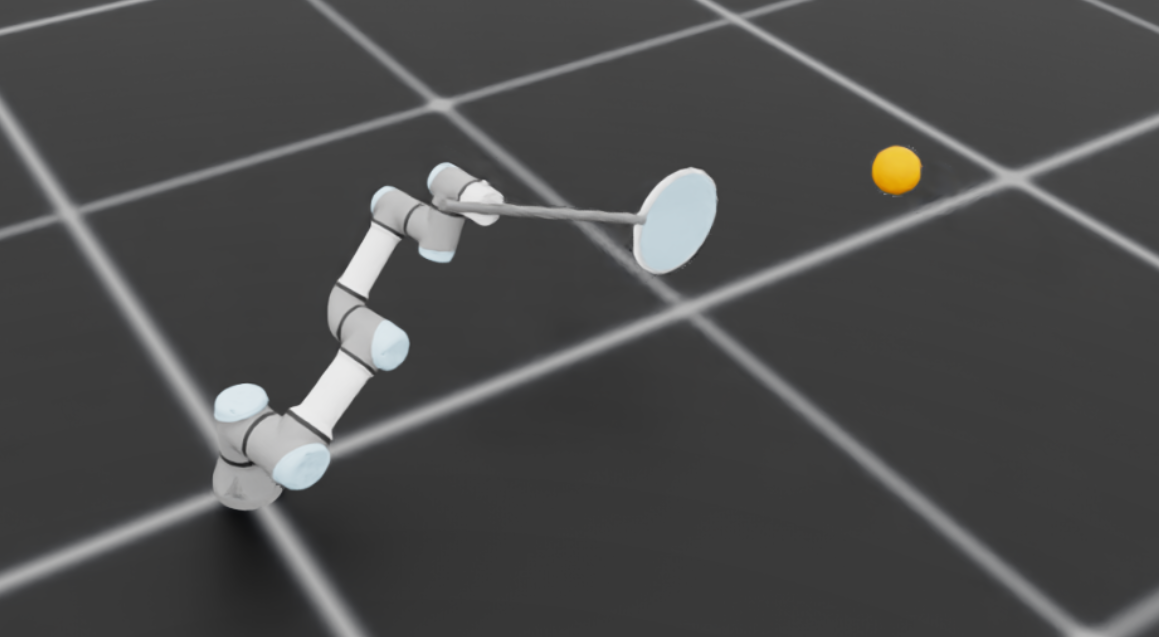
\includegraphics[width=3.60cm]{images/UR3e_Sim.png}};
  \node[plansub] at ($(SW)+(8.00,2.36)$)
    {séquences simulées\\apprentissage d'interception\\export de politique};

  \node[circle,fill=orangehot,draw=amber,line width=0.35pt,text=cream,
    font=\fontsize{7.2}{7.2}\selectfont\bfseries,minimum size=0.48cm]
    at ($(SW)+(11.62,6.68)$) {3};
  \node[planlabel,text width=2.84cm] at ($(SW)+(13.22,6.62)$) {UR3e réel\\boucle fermée};
  \node[anchor=center,opacity=0.68] at ($(SW)+(13.18,4.42)$)
    {\includegraphics[page=12,trim=4.1cm 0cm 4.1cm 0cm,clip,width=3.50cm]{RigonPresentation.pdf}};
  \draw[amber,opacity=0.90,line width=0.56pt]
    ($(SW)+(12.02,3.02)$) -- ($(SW)+(14.34,3.02)$);
  \draw[orangehot,opacity=0.72,line width=0.46pt]
    ($(SW)+(13.18,2.74)$) -- ($(SW)+(13.18,3.24)$);
  \node[plansub] at ($(SW)+(13.22,2.36)$)
    {contrôle du robot\\avec inférence};

  \draw[planarrow] ($(SW)+(4.98,4.42)$) -- ($(SW)+(5.78,4.42)$);
  \draw[planarrow] ($(SW)+(10.20,4.42)$) -- ($(SW)+(11.00,4.42)$);
  \node[
    anchor=south east,
    text=softcream,
    font=\fontsize{4.7}{5.0}\selectfont,
    opacity=0.75
  ] at ($(SW)+(15.50,0.40)$) {3 / 13};
\end{tikzpicture}

\newpage

\begin{tikzpicture}[remember picture,overlay]
  \path (current page.south west) coordinate (SW);
  \path (current page.north east) coordinate (NE);

  \shade[left color=deepbrown,right color=redbrown] (SW) rectangle (NE);
  \fill[rust,opacity=0.36]
    (SW) -- ($(SW)+(5.8,0)$) -- ($(NE)+(-5.1,0)$) -- ($(NE)+(-9.5,0)$) -- cycle;
  \fill[orangehot,opacity=0.18]
    ($(SW)+(0,0)$) -- ($(SW)+(2.6,0)$) -- ($(NE)+(-7.4,0)$) -- ($(NE)+(-10.7,0)$) -- cycle;
  \fill[deepbrown,opacity=0.28] (SW) rectangle (NE);

  \node[
    anchor=west,
    text=cream,
    font=\fontsize{20}{22}\selectfont\bfseries
  ] at ($(SW)+(0.72,8.20)$) {Pourquoi une caméra événementielle ?};
  \draw[orangehot,line width=0.85pt] ($(SW)+(0.74,7.88)$) -- ($(SW)+(7.30,7.88)$);
  \draw[amber,line width=0.40pt,opacity=0.75] ($(SW)+(0.74,7.75)$) -- ($(SW)+(4.10,7.75)$);

  \tikzset{
    videopanel/.style={
      fill=deepbrown,
      fill opacity=0.58,
      draw=orangehot,
      draw opacity=0.84,
      line width=0.55pt,
      rounded corners=5pt
    },
    reason/.style={
      fill=redbrown,
      fill opacity=0.74,
      draw=amber,
      draw opacity=0.58,
      line width=0.30pt,
      rounded corners=3pt
    }
  }

  \path[videopanel] ($(SW)+(0.74,1.02)$) rectangle ($(SW)+(9.56,7.12)$);
  \node[anchor=center,inner sep=0pt] at ($(SW)+(5.15,4.22)$)
    {\movie[externalviewer=false,showcontrols=true]{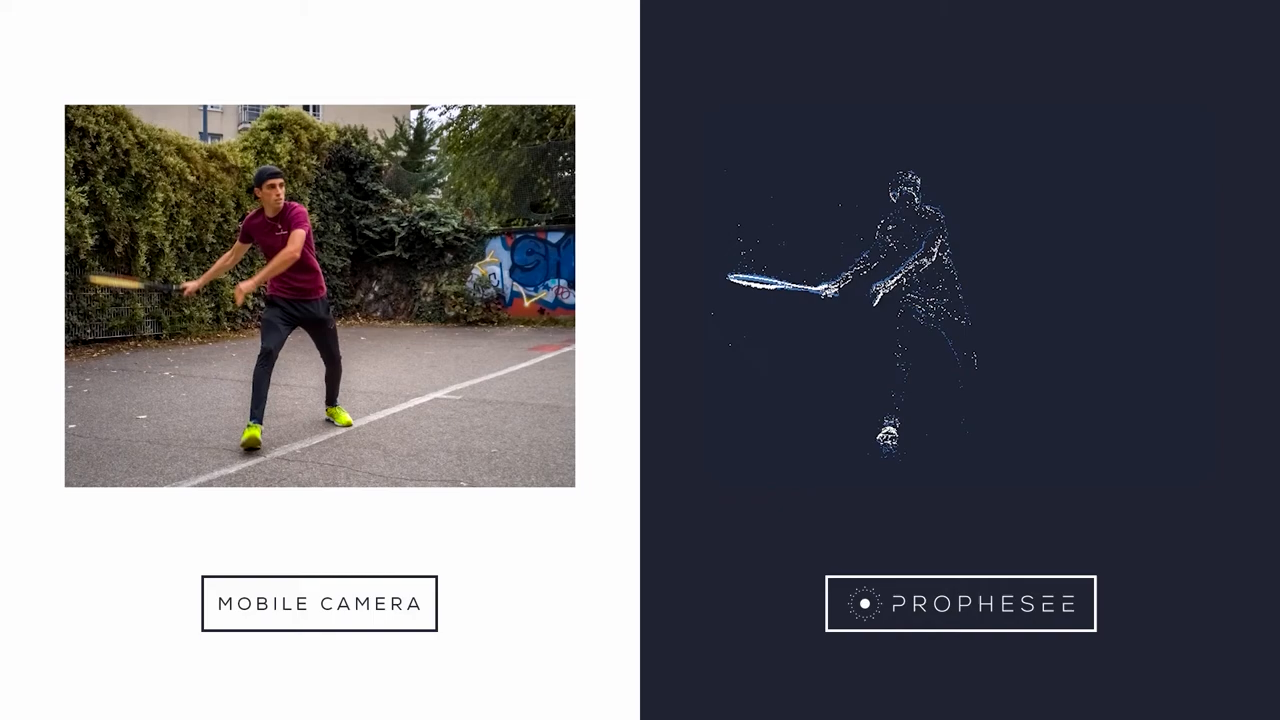
\includegraphics[width=8.08cm]{images/prophesee_event_camera_poster.png}}{video/prophesee_event_camera.mp4}};
  \fill[deepbrown,opacity=0.62] ($(SW)+(5.15,4.22)$) circle (0.42cm);
  \draw[amber,opacity=0.92,line width=0.55pt] ($(SW)+(5.15,4.22)$) circle (0.42cm);
  \fill[amber,opacity=0.96]
    ($(SW)+(5.03,3.99)$) -- ($(SW)+(5.03,4.45)$) -- ($(SW)+(5.41,4.22)$) -- cycle;

  \path[videopanel] ($(SW)+(10.10,1.02)$) rectangle ($(SW)+(15.28,7.12)$);
  \node[
    anchor=west,
    text=amber,
    font=\fontsize{8.0}{8.6}\selectfont\bfseries
  ] at ($(SW)+(10.44,6.74)$) {Pertinence pour l'interception};

  \path[reason] ($(SW)+(10.46,5.58)$) rectangle ($(SW)+(14.92,6.26)$);
  \node[anchor=center,text=cream,font=\fontsize{5.4}{5.9}\selectfont,text width=3.95cm,align=left]
    at ($(SW)+(12.69,5.92)$) {\textbf{Temps fin}\\chaque événement est daté};

  \path[reason] ($(SW)+(10.46,4.18)$) rectangle ($(SW)+(14.92,5.18)$);
  \node[anchor=center,text=cream,font=\fontsize{4.8}{5.3}\selectfont,text width=3.95cm,align=left]
    at ($(SW)+(12.69,4.68)$) {\textbf{Peu de données}\\image 640x480@60: \(\sim\)440 Mbit/s\\events 0,5 Mev/s: \(\sim\)20 Mbit/s};

  \path[reason] ($(SW)+(10.46,3.34)$) rectangle ($(SW)+(14.92,4.02)$);
  \node[anchor=center,text=cream,font=\fontsize{5.4}{5.9}\selectfont,text width=3.95cm,align=left]
    at ($(SW)+(12.69,3.68)$) {\textbf{Balle rapide}\\pas de flou};

  \node[
    anchor=center,
    text=cream,
    font=\fontsize{6.3}{7.0}\selectfont\bfseries,
    text width=4.15cm,
    align=center
  ] at ($(SW)+(12.70,1.48)$)
    {Objectif: garder une mesure exploitable malgré la vitesse};
  \node[
    anchor=south east,
    text=softcream,
    font=\fontsize{4.7}{5.0}\selectfont,
    opacity=0.75
  ] at ($(SW)+(15.50,0.40)$) {4 / 13};
\end{tikzpicture}

\newpage

\begin{tikzpicture}[remember picture,overlay]
  \path (current page.south west) coordinate (SW);
  \path (current page.north east) coordinate (NE);

  \shade[left color=deepbrown,right color=redbrown] (SW) rectangle (NE);
  \fill[rust,opacity=0.35]
    (SW) -- ($(SW)+(5.7,0)$) -- ($(NE)+(-5.0,0)$) -- ($(NE)+(-9.4,0)$) -- cycle;
  \fill[orangehot,opacity=0.18]
    ($(SW)+(0,0)$) -- ($(SW)+(2.7,0)$) -- ($(NE)+(-7.2,0)$) -- ($(NE)+(-10.6,0)$) -- cycle;
  \fill[deepbrown,opacity=0.28] (SW) rectangle (NE);

  \node[
    anchor=west,
    text=cream,
    font=\fontsize{20}{22}\selectfont\bfseries
  ] at ($(SW)+(0.72,8.20)$) {Calibration intrinsèque};
  \draw[orangehot,line width=0.85pt] ($(SW)+(0.74,7.88)$) -- ($(SW)+(5.55,7.88)$);
  \draw[amber,line width=0.40pt,opacity=0.75] ($(SW)+(0.74,7.75)$) -- ($(SW)+(3.05,7.75)$);

  \tikzset{
    calpanel/.style={
      fill=deepbrown,
      fill opacity=0.58,
      draw=orangehot,
      draw opacity=0.84,
      line width=0.55pt,
      rounded corners=5pt
    },
    calchip/.style={
      fill=redbrown,
      fill opacity=0.76,
      draw=amber,
      draw opacity=0.60,
      line width=0.30pt,
      rounded corners=3pt
    }
  }

  \path[calpanel] ($(SW)+(0.72,1.02)$) rectangle ($(SW)+(7.28,7.12)$);
  \node[anchor=west,text=amber,font=\fontsize{7.0}{7.6}\selectfont\bfseries]
    at ($(SW)+(1.02,6.78)$) {Mire clignotante sur écran};
  \node[anchor=center,inner sep=0pt] at ($(SW)+(4.00,4.02)$)
    {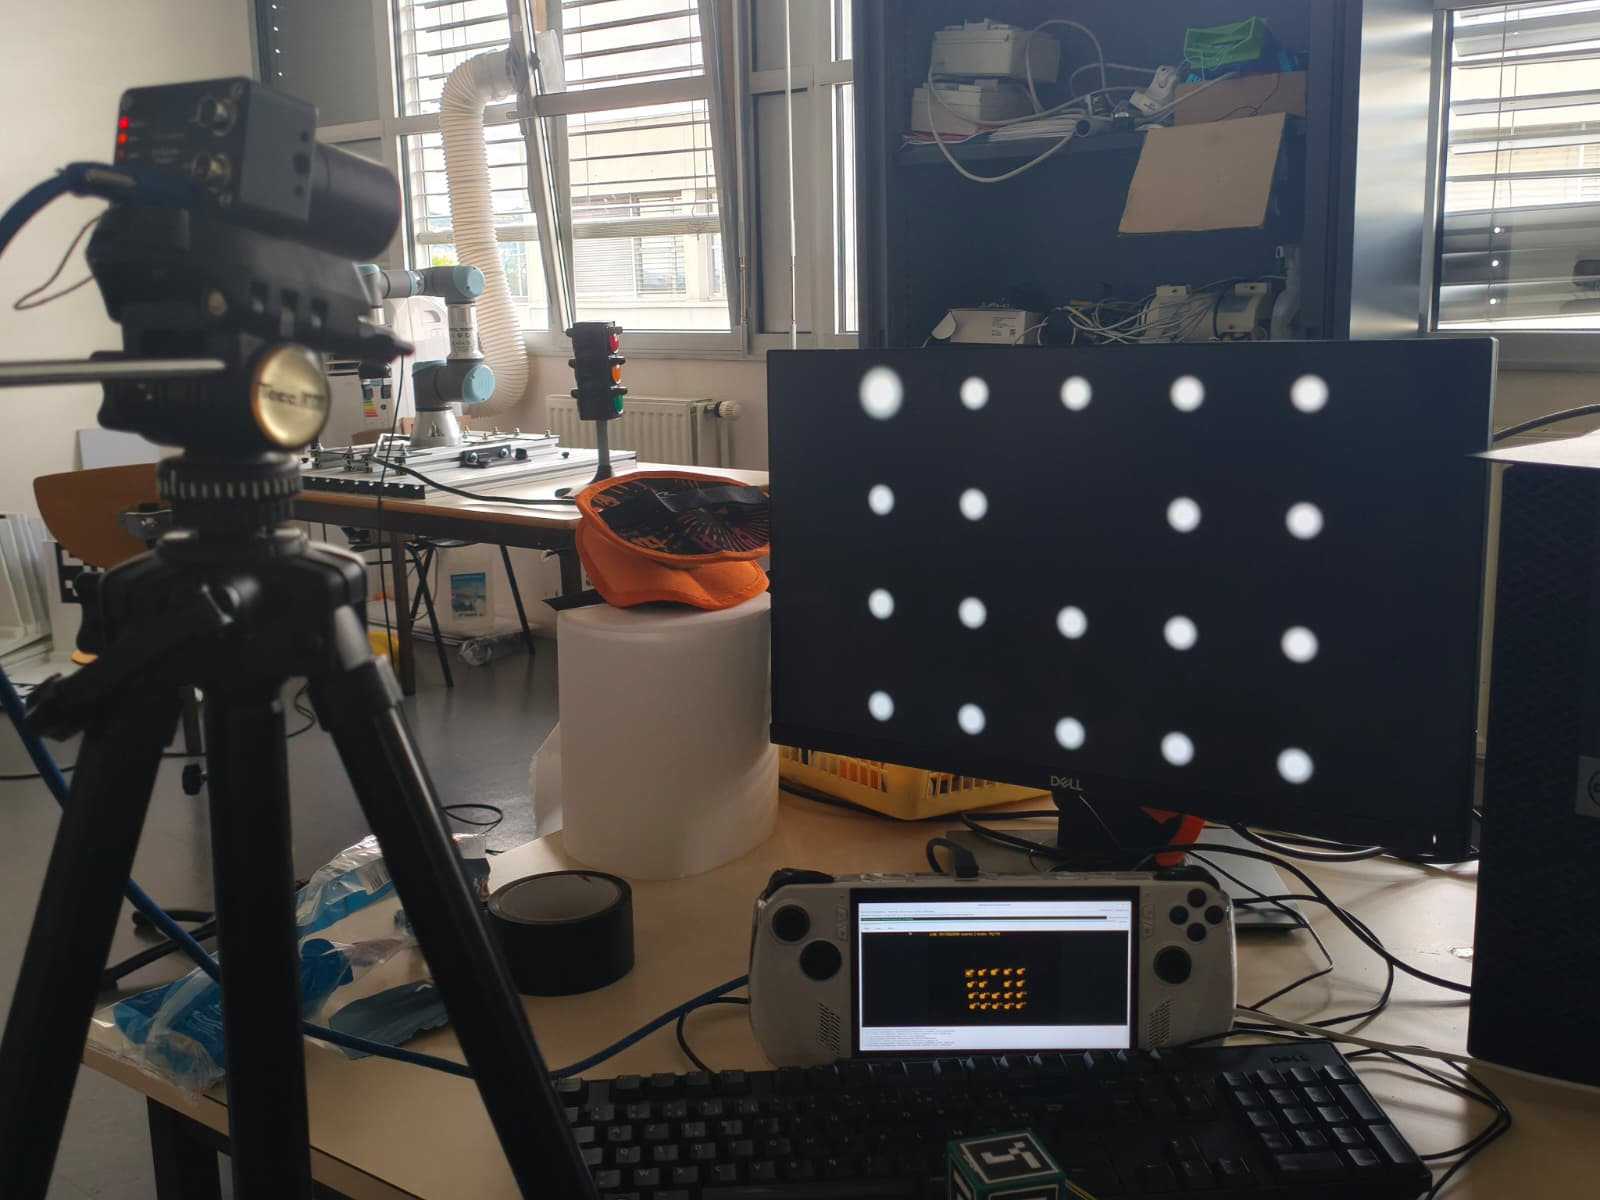
\includegraphics[width=5.95cm]{images/Calibration/Calibration_setup_ecran.jpeg}};
  \node[
    anchor=center,
    text=softcream,
    font=\fontsize{5.0}{5.5}\selectfont,
    text width=5.65cm,
    align=center
  ] at ($(SW)+(4.00,1.45)$)
    {disques lumineux clignotants pour générer des événements nets};

  \path[calpanel] ($(SW)+(7.72,4.16)$) rectangle ($(SW)+(15.28,7.12)$);
  \node[anchor=west,text=amber,font=\fontsize{7.0}{7.6}\selectfont\bfseries]
    at ($(SW)+(8.02,6.78)$) {Extraction des points};
  \node[anchor=center,inner sep=0pt] at ($(SW)+(10.12,5.36)$)
    {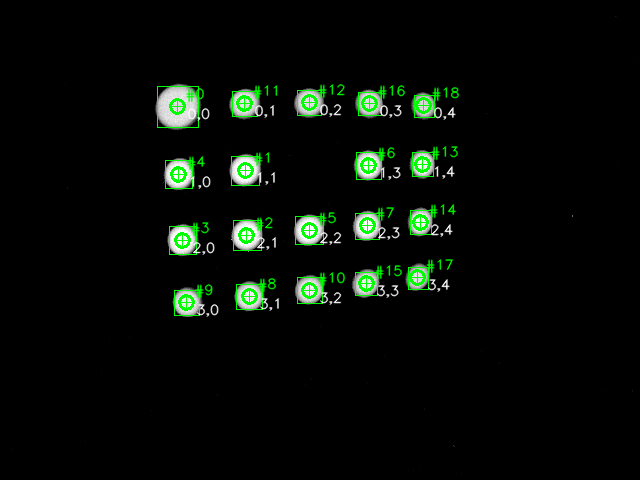
\includegraphics[width=2.82cm]{images/Calibration/mire_overlay_vue_1.png}};
  \node[
    anchor=west,
    text=softcream,
    font=\fontsize{5.0}{5.5}\selectfont,
    text width=2.00cm,
    align=left
  ] at ($(SW)+(12.22,5.42)$)
    {19 centres\\associés\\à la grille};

  \path[calpanel] ($(SW)+(7.72,1.02)$) rectangle ($(SW)+(15.28,3.76)$);
  \node[anchor=west,text=amber,font=\fontsize{7.0}{7.6}\selectfont\bfseries]
    at ($(SW)+(8.02,3.42)$) {Paramètres obtenus};

  \path[calchip] ($(SW)+(8.04,2.50)$) rectangle ($(SW)+(11.30,3.12)$);
  \node[anchor=center,text=cream,font=\fontsize{5.5}{6.0}\selectfont\bfseries]
    at ($(SW)+(9.67,2.81)$) {32 vues | RMS 0.189 px};

  \node[
    anchor=west,
    text=cream,
    font=\fontsize{5.6}{6.2}\selectfont,
    text width=3.55cm,
    align=left
  ] at ($(SW)+(8.08,1.88)$)
    {\(\displaystyle
      K \simeq
      \left[
      \begin{array}{ccc}
        526.3 & 0 & 330.9\\
        0 & 525.6 & 242.2\\
        0 & 0 & 1
      \end{array}
      \right]
    \)};

  \node[
    anchor=west,
    text=softcream,
    font=\fontsize{5.4}{5.9}\selectfont,
    text width=3.25cm,
    align=left
  ] at ($(SW)+(11.72,2.12)$)
    {\textbf{Distorsion}\\\(k_1 \simeq -0.403\)\\\(k_2 \simeq 0.167\)\\\(p_1=p_2=k_3=0\)};
  \node[
    anchor=south east,
    text=softcream,
    font=\fontsize{4.7}{5.0}\selectfont,
    opacity=0.75
  ] at ($(SW)+(15.50,0.40)$) {5 / 13};
\end{tikzpicture}

\newpage

\begin{tikzpicture}[remember picture,overlay]
  \path (current page.south west) coordinate (SW);
  \path (current page.north east) coordinate (NE);

  \shade[left color=deepbrown,right color=redbrown] (SW) rectangle (NE);
  \fill[rust,opacity=0.35]
    (SW) -- ($(SW)+(5.7,0)$) -- ($(NE)+(-5.0,0)$) -- ($(NE)+(-9.4,0)$) -- cycle;
  \fill[orangehot,opacity=0.18]
    ($(SW)+(0,0)$) -- ($(SW)+(2.7,0)$) -- ($(NE)+(-7.2,0)$) -- ($(NE)+(-10.6,0)$) -- cycle;
  \fill[deepbrown,opacity=0.28] (SW) rectangle (NE);

  \node[
    anchor=west,
    text=cream,
    font=\fontsize{20}{22}\selectfont\bfseries
  ] at ($(SW)+(0.72,8.20)$) {Calibration extrinsèque};
  \draw[orangehot,line width=0.85pt] ($(SW)+(0.74,7.88)$) -- ($(SW)+(5.70,7.88)$);
  \draw[amber,line width=0.40pt,opacity=0.75] ($(SW)+(0.74,7.75)$) -- ($(SW)+(3.12,7.75)$);

  \tikzset{
    extpanel/.style={
      fill=deepbrown,
      fill opacity=0.58,
      draw=orangehot,
      draw opacity=0.84,
      line width=0.55pt,
      rounded corners=5pt
    }
  }

  \path[extpanel] ($(SW)+(0.72,0.86)$) rectangle ($(SW)+(6.78,7.12)$);
  \node[anchor=center,inner sep=0pt] at ($(SW)+(3.75,3.99)$)
    {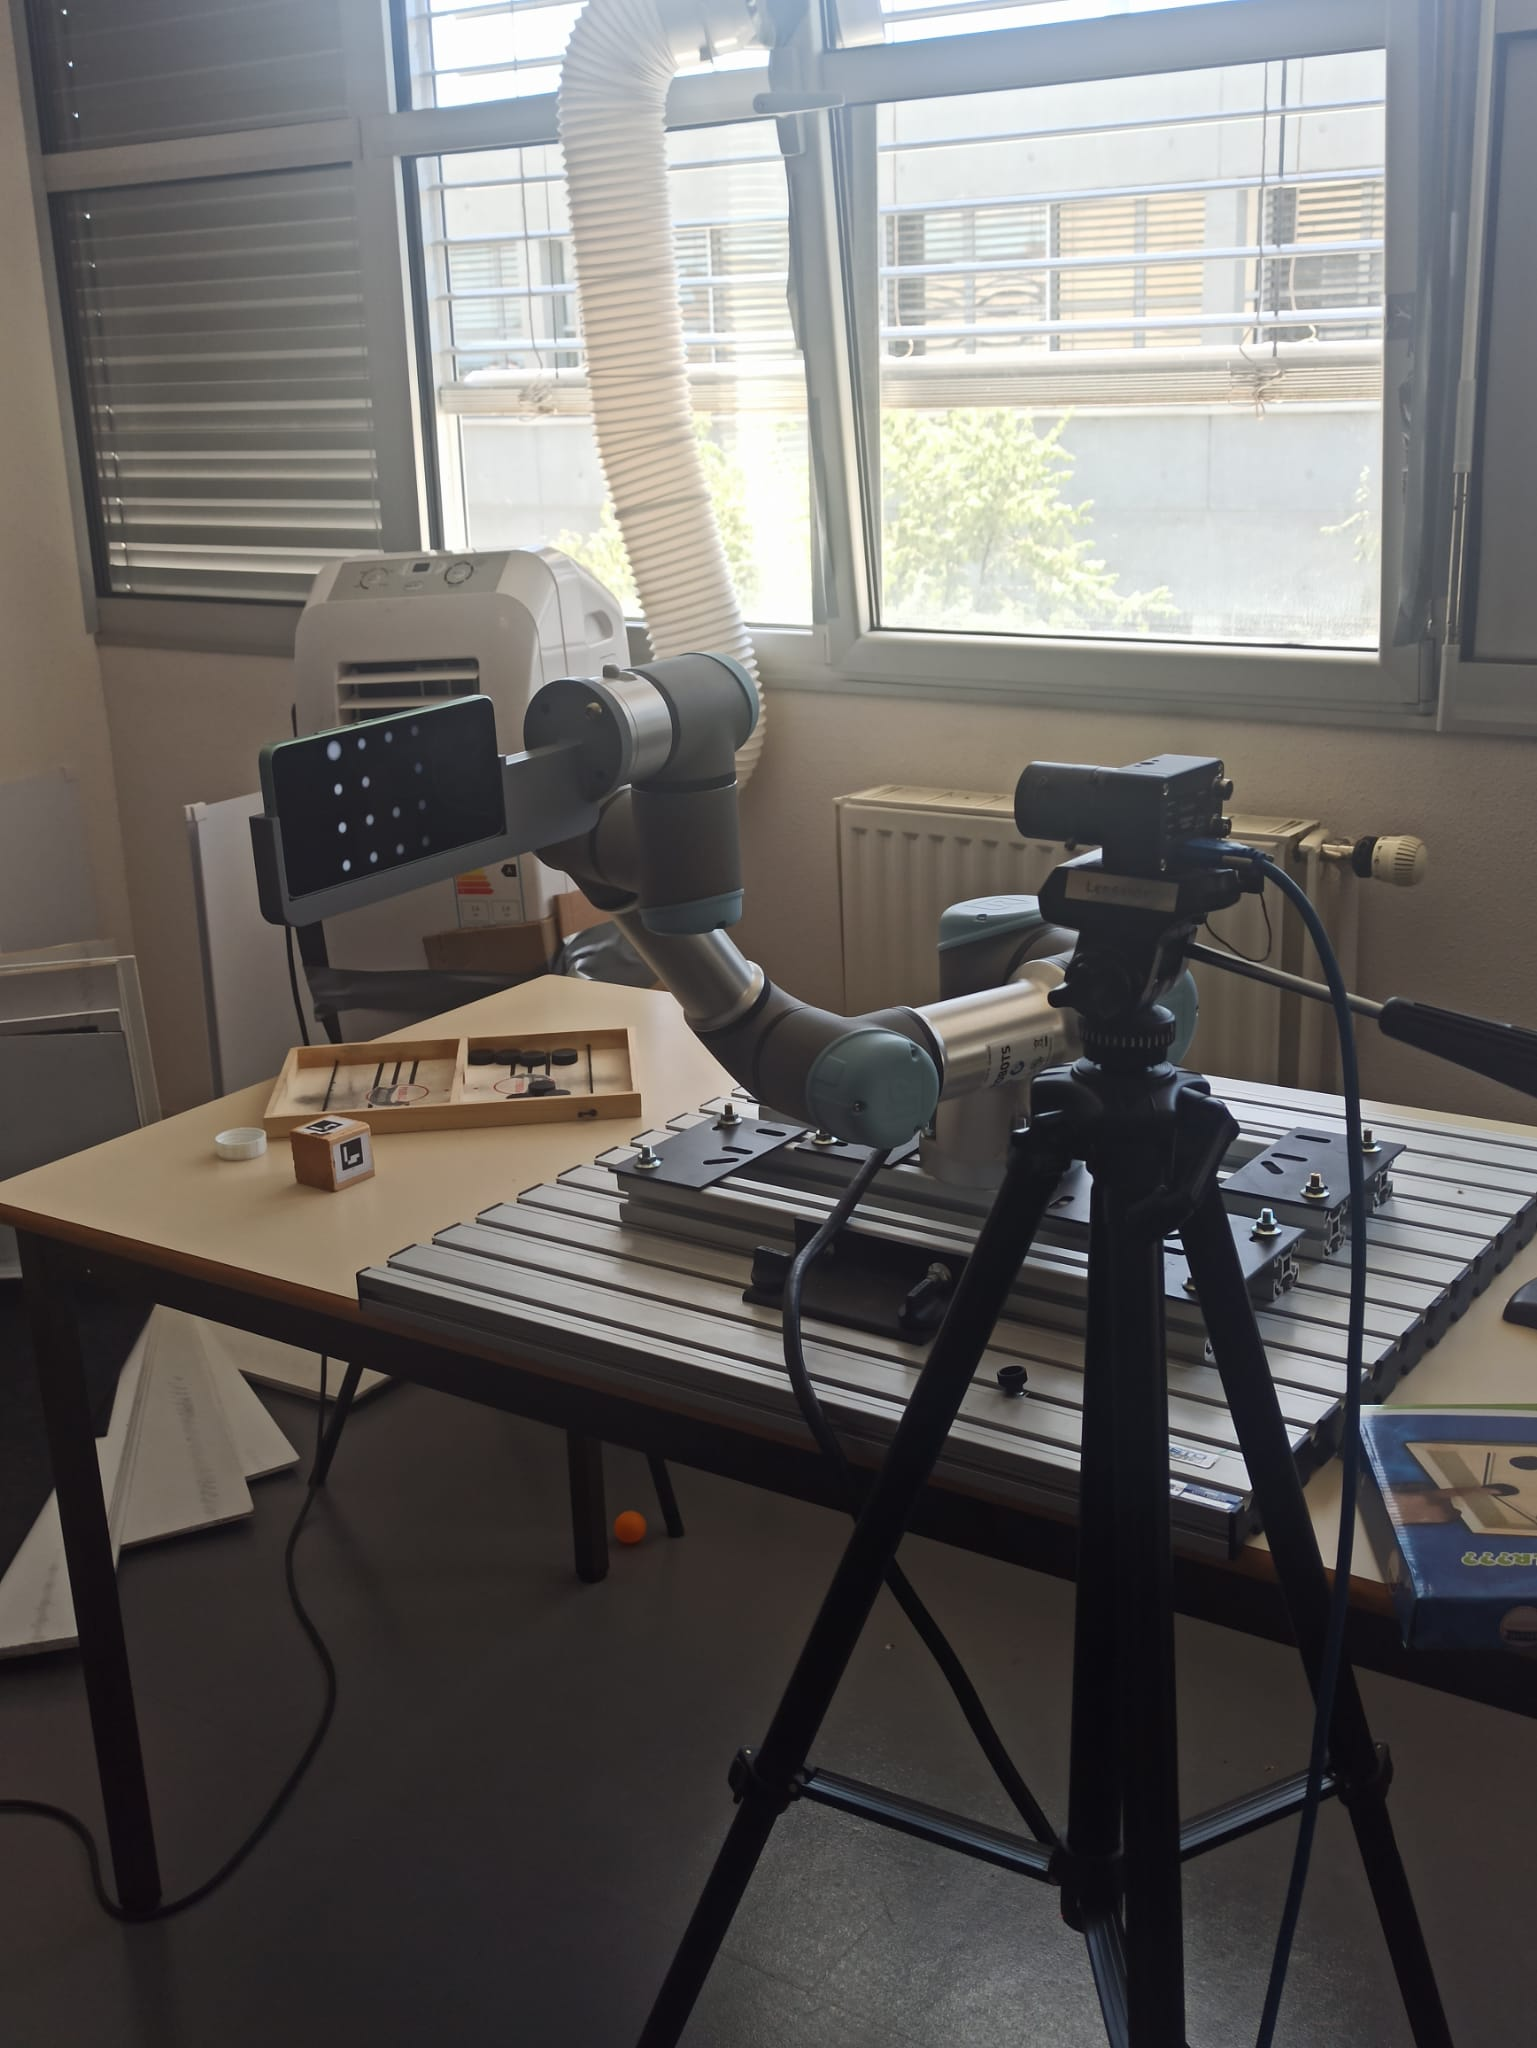
\includegraphics[height=5.82cm]{images/Calibration/Smartphone_Sur_Support_vue_coté.jpeg}};

  \path[extpanel] ($(SW)+(7.18,0.86)$) rectangle ($(SW)+(15.28,7.12)$);
  \node[anchor=center,inner sep=0pt] at ($(SW)+(11.23,3.99)$)
    {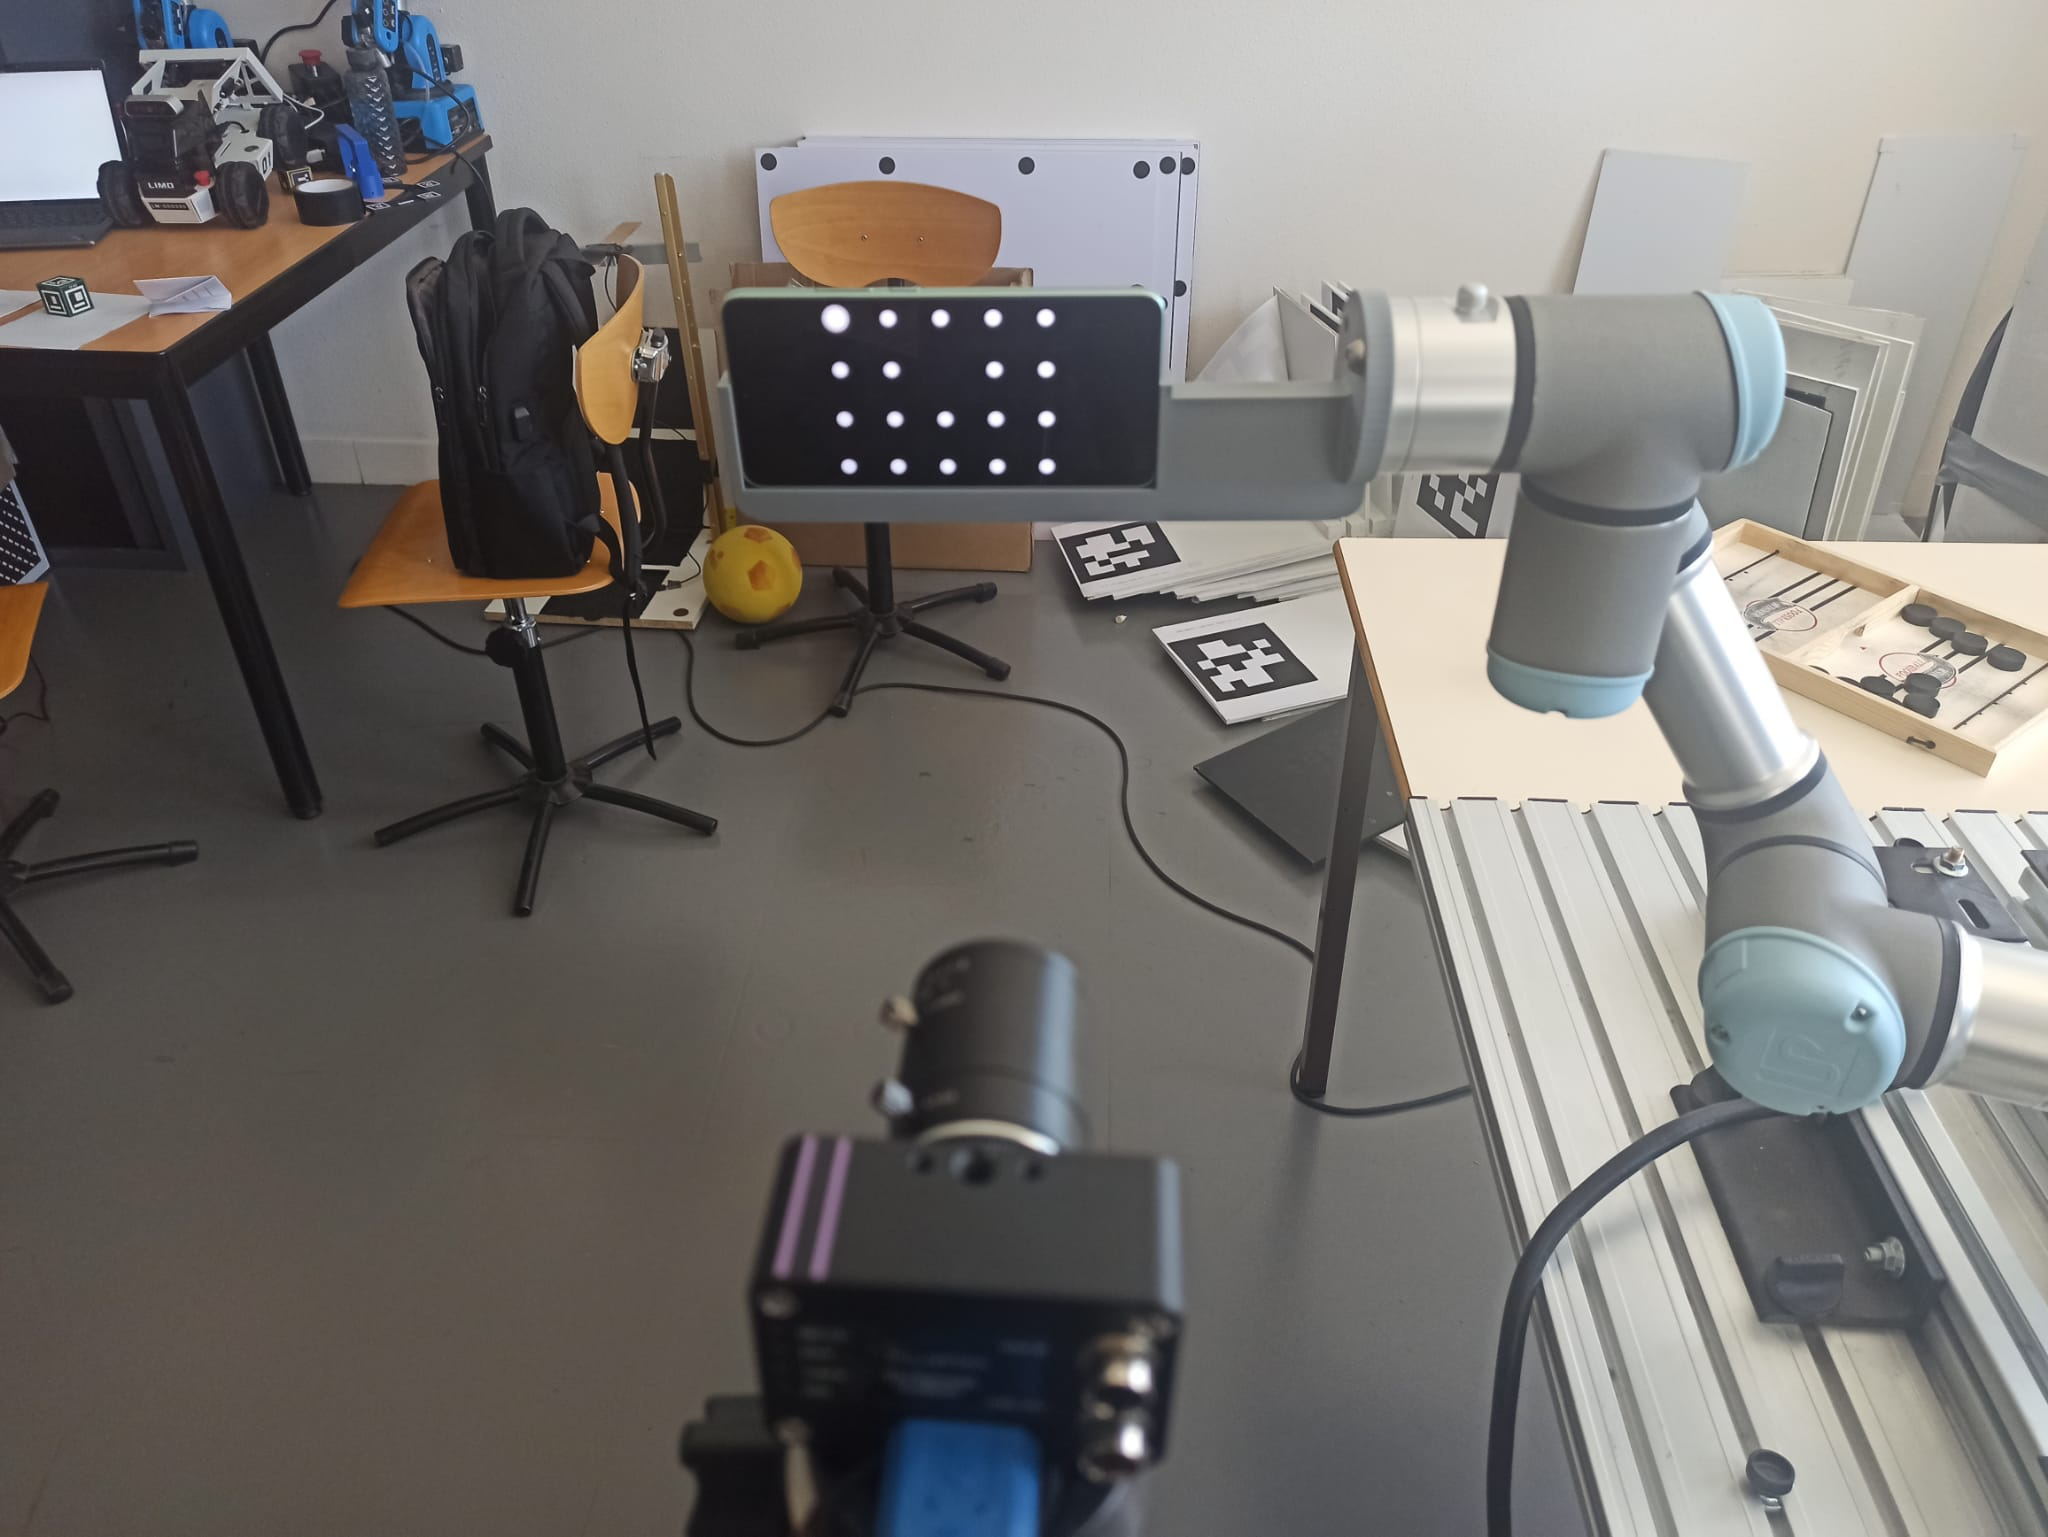
\includegraphics[width=7.46cm]{images/Calibration/Smartphone_Sur_Support.jpeg}};
  \node[
    anchor=south east,
    text=softcream,
    font=\fontsize{4.7}{5.0}\selectfont,
    opacity=0.75
  ] at ($(SW)+(15.50,0.40)$) {6 / 13};
\end{tikzpicture}

\newpage

\begin{tikzpicture}[remember picture,overlay]
  \path (current page.south west) coordinate (SW);
  \path (current page.north east) coordinate (NE);

  \shade[left color=deepbrown,right color=redbrown] (SW) rectangle (NE);
  \fill[rust,opacity=0.35]
    (SW) -- ($(SW)+(5.7,0)$) -- ($(NE)+(-5.0,0)$) -- ($(NE)+(-9.4,0)$) -- cycle;
  \fill[orangehot,opacity=0.18]
    ($(SW)+(0,0)$) -- ($(SW)+(2.7,0)$) -- ($(NE)+(-7.2,0)$) -- ($(NE)+(-10.6,0)$) -- cycle;
  \fill[deepbrown,opacity=0.28] (SW) rectangle (NE);

  \node[
    anchor=west,
    text=cream,
    font=\fontsize{20}{22}\selectfont\bfseries
  ] at ($(SW)+(0.72,8.20)$) {Algorithme d'ajustement de cercle};
  \draw[orangehot,line width=0.85pt] ($(SW)+(0.74,7.88)$) -- ($(SW)+(8.20,7.88)$);
  \draw[amber,line width=0.40pt,opacity=0.75] ($(SW)+(0.74,7.75)$) -- ($(SW)+(4.45,7.75)$);

  \tikzset{
    circlepanel/.style={
      fill=deepbrown,
      fill opacity=0.58,
      draw=orangehot,
      draw opacity=0.84,
      line width=0.55pt,
      rounded corners=5pt
    },
    circlechip/.style={
      fill=redbrown,
      fill opacity=0.78,
      draw=amber,
      draw opacity=0.62,
      line width=0.30pt,
      rounded corners=3pt,
      text=cream,
      align=center,
      font=\fontsize{4.8}{5.3}\selectfont\bfseries,
      minimum height=0.58cm
    },
    circlearrow/.style={-{Latex[length=1.4mm]},draw=amber,opacity=0.88,line width=0.42pt}
  }

  \path[circlepanel] ($(SW)+(0.72,4.52)$) rectangle ($(SW)+(7.54,7.12)$);
  \node[anchor=west,text=amber,font=\fontsize{7.0}{7.6}\selectfont\bfseries]
    at ($(SW)+(1.02,6.78)$) {Sortie 2D};
  \node[anchor=east,text=softcream,font=\fontsize{4.8}{5.2}\selectfont]
    at ($(SW)+(7.20,6.78)$) {cluster + cercle retenu};
  \node[anchor=center,inner sep=0pt] at ($(SW)+(4.13,5.62)$)
    {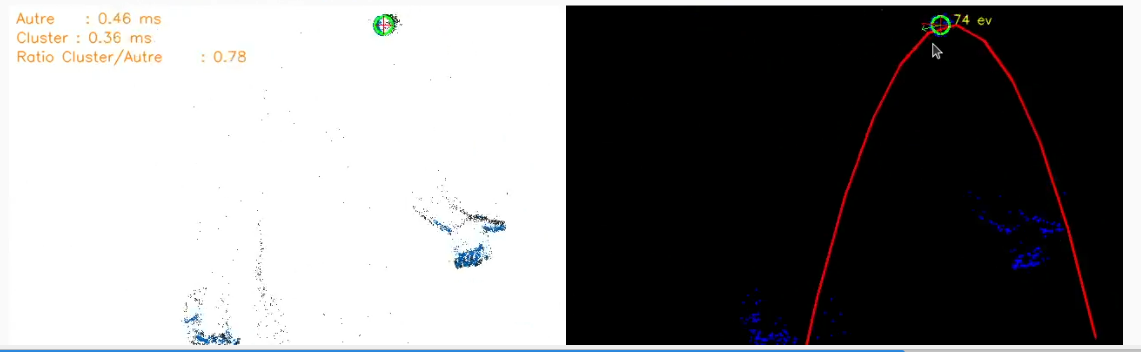
\includegraphics[width=6.34cm]{images/Algo_Cricle_Fitting/Sortie_algo_2D.png}};

  \path[circlepanel] ($(SW)+(0.72,1.02)$) rectangle ($(SW)+(7.54,4.18)$);
  \node[anchor=west,text=amber,font=\fontsize{7.0}{7.6}\selectfont\bfseries]
    at ($(SW)+(1.02,3.86)$) {Chaîne de calcul};

  \node[circlechip,text width=1.54cm] (w) at ($(SW)+(1.80,3.10)$) {fenêtre\\temporelle};
  \node[circlechip,text width=1.54cm] (d) at ($(SW)+(4.13,3.10)$) {DBSCAN\\cluster balle};
  \node[circlechip,text width=1.54cm] (c) at ($(SW)+(6.46,3.10)$) {cercle 2D\\\((u,v,r)\)};
  \node[circlechip,text width=1.64cm] (p) at ($(SW)+(2.95,2.00)$) {rayon \(\rightarrow\)\\profondeur};
  \node[circlechip,text width=1.64cm] (t) at ($(SW)+(5.35,2.00)$) {régression\\trajectoire};

  \draw[circlearrow] (w.east) -- (d.west);
  \draw[circlearrow] (d.east) -- (c.west);
  \draw[circlearrow] (c.south) -- ($(c.south)+(0,-0.23)$) -- ($(p.north)+(0,0.23)$) -- (p.north);
  \draw[circlearrow] (p.east) -- (t.west);

  \node[
    anchor=center,
    text=cream,
    font=\fontsize{6.0}{6.5}\selectfont\bfseries,
    text width=5.88cm,
    align=center
  ] at ($(SW)+(4.13,1.33)$)
    {\(\displaystyle Z=\frac{f_x R}{r}\) \quad puis projection inverse en 3D};

  \path[circlepanel] ($(SW)+(7.88,1.02)$) rectangle ($(SW)+(15.28,7.12)$);
  \node[anchor=west,text=amber,font=\fontsize{7.0}{7.6}\selectfont\bfseries]
    at ($(SW)+(8.18,6.78)$) {Estimation 3D};
  \node[anchor=east,text=softcream,font=\fontsize{4.8}{5.2}\selectfont]
    at ($(SW)+(14.92,6.78)$) {points validés + parabole};
  \node[anchor=center,inner sep=0pt] at ($(SW)+(11.58,4.35)$)
    {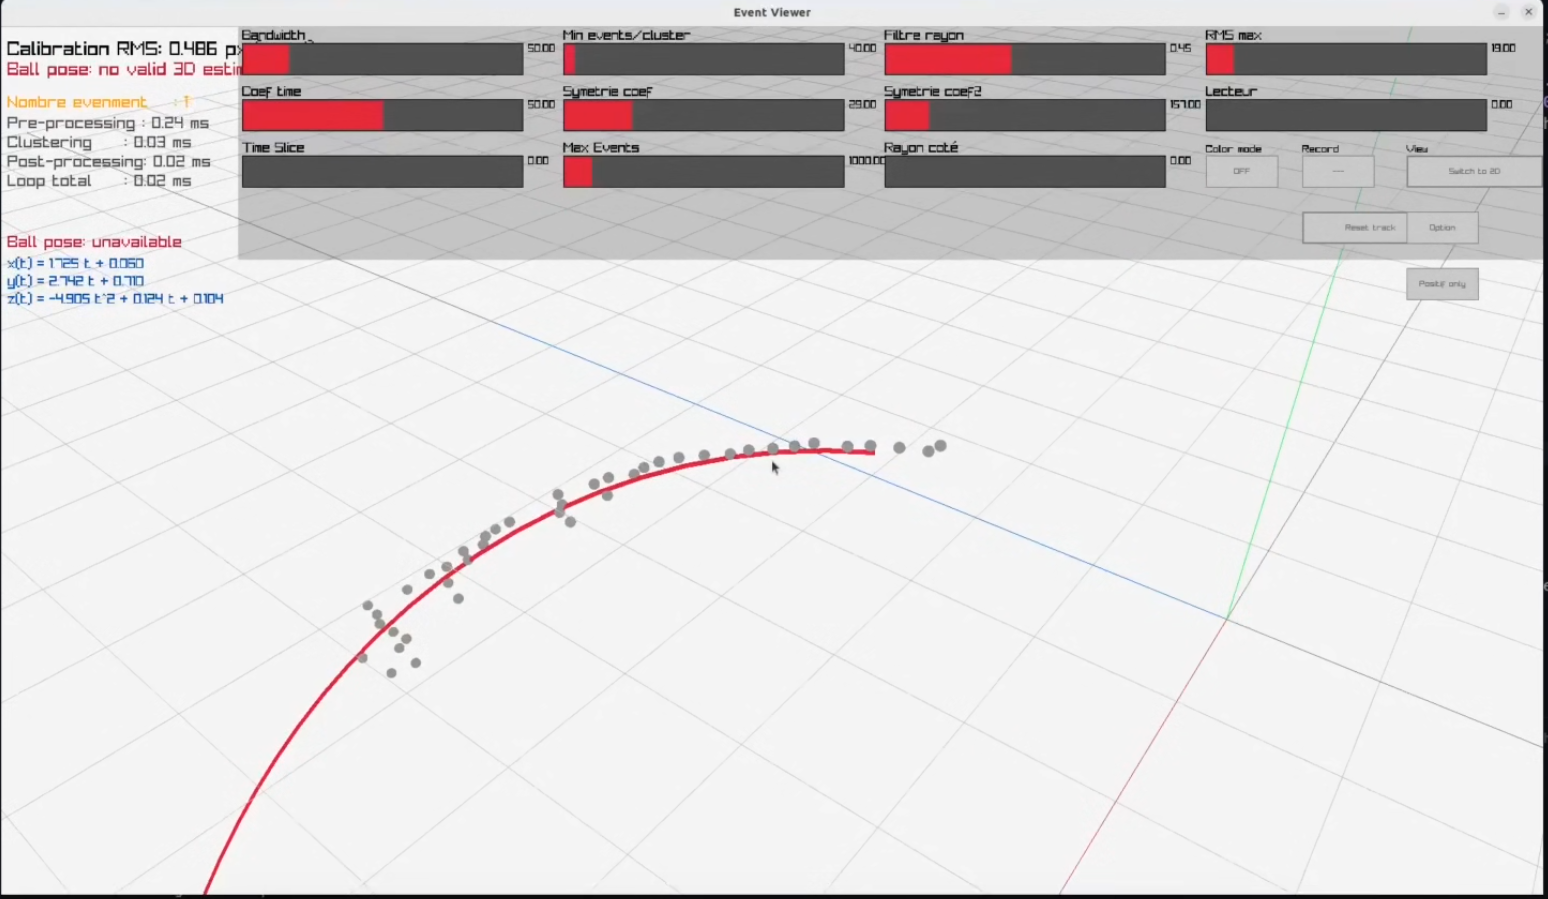
\includegraphics[width=6.92cm]{images/Algo_Cricle_Fitting/3D_estimation.png}};

  \fill[orangehot,opacity=0.17,rounded corners=3pt]
    ($(SW)+(8.32,1.28)$) rectangle ($(SW)+(14.82,1.86)$);
  \node[
    anchor=center,
    text=cream,
    font=\fontsize{5.5}{6.0}\selectfont\bfseries,
    text width=5.86cm,
    align=center
  ] at ($(SW)+(11.57,1.57)$)
    {Projection 2D supposée circulaire};
  \node[
    anchor=south east,
    text=softcream,
    font=\fontsize{4.7}{5.0}\selectfont,
    opacity=0.75
  ] at ($(SW)+(15.50,0.40)$) {7 / 13};
\end{tikzpicture}

\newpage

\begin{tikzpicture}[remember picture,overlay]
  \path (current page.south west) coordinate (SW);
  \path (current page.north east) coordinate (NE);

  \shade[left color=deepbrown,right color=redbrown] (SW) rectangle (NE);
  \fill[rust,opacity=0.35]
    (SW) -- ($(SW)+(5.7,0)$) -- ($(NE)+(-5.0,0)$) -- ($(NE)+(-9.4,0)$) -- cycle;
  \fill[orangehot,opacity=0.18]
    ($(SW)+(0,0)$) -- ($(SW)+(2.7,0)$) -- ($(NE)+(-7.2,0)$) -- ($(NE)+(-10.6,0)$) -- cycle;
  \fill[deepbrown,opacity=0.28] (SW) rectangle (NE);

  \node[
    anchor=west,
    text=cream,
    font=\fontsize{20}{22}\selectfont\bfseries
  ] at ($(SW)+(0.72,8.20)$) {Circle fitting : problème rencontré};
  \draw[orangehot,line width=0.85pt] ($(SW)+(0.74,7.88)$) -- ($(SW)+(8.75,7.88)$);
  \draw[amber,line width=0.40pt,opacity=0.75] ($(SW)+(0.74,7.75)$) -- ($(SW)+(4.70,7.75)$);

  \tikzset{
    problempanel/.style={
      fill=deepbrown,
      fill opacity=0.58,
      draw=orangehot,
      draw opacity=0.84,
      line width=0.55pt,
      rounded corners=5pt
    },
    problemchip/.style={
      fill=redbrown,
      fill opacity=0.80,
      draw=amber,
      draw opacity=0.66,
      line width=0.32pt,
      rounded corners=3pt,
      text=cream,
      align=center,
      font=\fontsize{4.55}{4.95}\selectfont\bfseries,
      minimum height=0.40cm
    }
  }

  \path[problempanel] ($(SW)+(0.72,0.96)$) rectangle ($(SW)+(8.42,7.12)$);
  \node[anchor=west,text=amber,font=\fontsize{7.0}{7.6}\selectfont\bfseries]
    at ($(SW)+(1.02,6.78)$) {Diagnostic 3D};
  \node[anchor=east,text=softcream,font=\fontsize{4.8}{5.2}\selectfont]
    at ($(SW)+(8.06,6.78)$) {trajectoire estimée instable};
  \node[anchor=center,inner sep=0pt] at ($(SW)+(4.57,4.22)$)
    {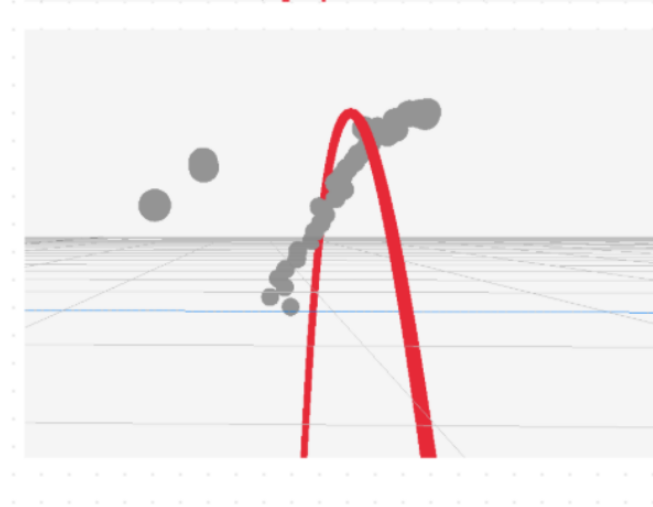
\includegraphics[width=6.08cm]{images/Algo_Cricle_Fitting/3D_blem1.png}};
  \node[
    anchor=center,
    text=cream,
    font=\fontsize{5.1}{5.6}\selectfont,
    text width=6.75cm,
    align=center
  ] at ($(SW)+(4.57,1.30)$)
    {Les points 3D ne suivent plus le plan attendu : la profondeur est ramenée artificiellement vers la caméra.};

  \path[problempanel] ($(SW)+(8.78,4.32)$) rectangle ($(SW)+(15.28,7.12)$);
  \node[anchor=west,text=amber,font=\fontsize{7.0}{7.6}\selectfont\bfseries]
    at ($(SW)+(9.08,6.78)$) {Sensibilité du rayon};
  \node[
    anchor=center,
    text=cream,
    font=\fontsize{9.0}{9.8}\selectfont\bfseries,
    text width=5.64cm,
    align=center
  ] at ($(SW)+(12.03,6.08)$)
    {\(\displaystyle Z=\frac{f_x R}{r_{px}}\)};
  \node[
    anchor=center,
    text=softcream,
    font=\fontsize{5.25}{5.75}\selectfont,
    text width=5.70cm,
    align=center
  ] at ($(SW)+(12.03,5.45)$)
    {\(1~px\) sur \(r_{px}\) \(\Rightarrow\) erreur \(\approx Z/r_{px}\approx14~cm\)};
  \node[problemchip,text width=1.58cm] at ($(SW)+(10.46,4.86)$) {\(r_{px}\) petit\\loin caméra};
  \node[problemchip,text width=1.68cm] at ($(SW)+(13.60,4.86)$) {erreur \(Z\)\\amplifiée};

  \path[problempanel] ($(SW)+(8.78,0.96)$) rectangle ($(SW)+(15.28,4.04)$);
  \node[anchor=west,text=amber,font=\fontsize{7.0}{7.6}\selectfont\bfseries]
    at ($(SW)+(9.08,3.70)$) {Cause observée};
  \node[
    anchor=west,
    text=cream,
    font=\fontsize{5.75}{6.35}\selectfont,
    text width=5.65cm,
    align=left
  ] at ($(SW)+(9.12,3.04)$)
    {\textbf{Balle rapide} : les événements forment une traînée, pas un contour circulaire net.};
  \node[
    anchor=west,
    text=cream,
    font=\fontsize{5.75}{6.35}\selectfont,
    text width=5.65cm,
    align=left
  ] at ($(SW)+(9.12,2.18)$)
    {\textbf{Rayon surestimé} : le cercle englobe une zone trop large.};
  \node[
    anchor=west,
    text=cream,
    font=\fontsize{5.75}{6.35}\selectfont,
    text width=5.65cm,
    align=left
  ] at ($(SW)+(9.12,1.32)$)
    {\textbf{Profondeur sous-estimée} : \(r_{px}\uparrow\), donc \(Z\downarrow\).};
  \node[
    anchor=south east,
    text=softcream,
    font=\fontsize{4.7}{5.0}\selectfont,
    opacity=0.75
  ] at ($(SW)+(15.50,0.40)$) {8 / 13};
\end{tikzpicture}

\newpage

\begin{tikzpicture}[remember picture,overlay]
  \path (current page.south west) coordinate (SW);
  \path (current page.north east) coordinate (NE);

  \shade[left color=deepbrown,right color=redbrown] (SW) rectangle (NE);
  \fill[rust,opacity=0.35]
    (SW) -- ($(SW)+(5.7,0)$) -- ($(NE)+(-5.0,0)$) -- ($(NE)+(-9.4,0)$) -- cycle;
  \fill[orangehot,opacity=0.18]
    ($(SW)+(0,0)$) -- ($(SW)+(2.7,0)$) -- ($(NE)+(-7.2,0)$) -- ($(NE)+(-10.6,0)$) -- cycle;
  \fill[deepbrown,opacity=0.28] (SW) rectangle (NE);

  \node[
    anchor=west,
    text=cream,
    font=\fontsize{20}{22}\selectfont\bfseries
  ] at ($(SW)+(0.72,8.20)$) {Génération d'événements};
  \draw[orangehot,line width=0.85pt] ($(SW)+(0.74,7.88)$) -- ($(SW)+(7.05,7.88)$);
  \draw[amber,line width=0.40pt,opacity=0.75] ($(SW)+(0.74,7.75)$) -- ($(SW)+(4.06,7.75)$);

  \tikzset{
    v2epanel/.style={
      fill=deepbrown,
      fill opacity=0.58,
      draw=orangehot,
      draw opacity=0.84,
      line width=0.55pt,
      rounded corners=5pt
    }
  }

  \path[v2epanel] ($(SW)+(0.72,1.02)$) rectangle ($(SW)+(15.28,7.12)$);
  \node[anchor=center,inner sep=0pt] at ($(SW)+(8.00,4.12)$)
    {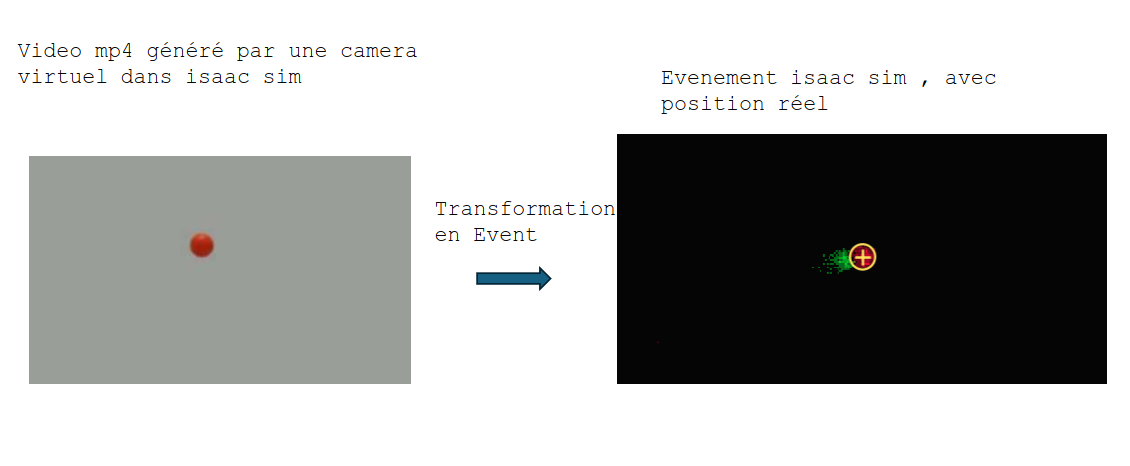
\includegraphics[width=13.95cm]{images/V2e.png}};

  \fill[orangehot,opacity=0.15,rounded corners=3pt]
    ($(SW)+(3.62,0.36)$) rectangle ($(SW)+(12.38,0.78)$);
  \node[
    anchor=center,
    text=cream,
    font=\fontsize{5.05}{5.5}\selectfont\bfseries,
    text width=8.20cm,
    align=center
  ] at ($(SW)+(8.00,0.57)$)
    {Simulation contrôlée : flux événementiel et position réelle de la balle.};
  \node[
    anchor=south east,
    text=softcream,
    font=\fontsize{4.7}{5.0}\selectfont,
    opacity=0.75
  ] at ($(SW)+(15.50,0.40)$) {9 / 13};
\end{tikzpicture}

\newpage

\begin{tikzpicture}[remember picture,overlay]
  \path (current page.south west) coordinate (SW);
  \path (current page.north east) coordinate (NE);

  \shade[left color=deepbrown,right color=redbrown] (SW) rectangle (NE);
  \fill[rust,opacity=0.35]
    (SW) -- ($(SW)+(5.7,0)$) -- ($(NE)+(-5.0,0)$) -- ($(NE)+(-9.4,0)$) -- cycle;
  \fill[orangehot,opacity=0.18]
    ($(SW)+(0,0)$) -- ($(SW)+(2.7,0)$) -- ($(NE)+(-7.2,0)$) -- ($(NE)+(-10.6,0)$) -- cycle;
  \fill[deepbrown,opacity=0.28] (SW) rectangle (NE);

  \node[
    anchor=west,
    text=cream,
    font=\fontsize{20}{22}\selectfont\bfseries
  ] at ($(SW)+(0.72,8.20)$) {Méthode Trace};
  \draw[orangehot,line width=0.85pt] ($(SW)+(0.74,7.88)$) -- ($(SW)+(4.35,7.88)$);
  \draw[amber,line width=0.40pt,opacity=0.75] ($(SW)+(0.74,7.75)$) -- ($(SW)+(2.62,7.75)$);

  \tikzset{
    tracepanel/.style={
      fill=deepbrown,
      fill opacity=0.58,
      draw=orangehot,
      draw opacity=0.84,
      line width=0.55pt,
      rounded corners=5pt
    }
  }

  \path[tracepanel] ($(SW)+(0.72,1.02)$) rectangle ($(SW)+(8.62,7.12)$);
  \node[anchor=west,text=amber,font=\fontsize{7.0}{7.6}\selectfont\bfseries]
    at ($(SW)+(1.02,6.78)$) {Ruban événementiel};
  \node[anchor=east,text=softcream,font=\fontsize{4.8}{5.2}\selectfont]
    at ($(SW)+(8.26,6.78)$) {bords + médiane + largeurs};
  \node[anchor=center,inner sep=0pt] at ($(SW)+(4.67,4.28)$)
    {
\includegraphics[width=7.05cm,trim=135 120 150 235,clip]{\detokenize{images/Algo_Trace/Screenshot from 2026-06-04 17-32-17.png}}};

  \fill[orangehot,opacity=0.15,rounded corners=3pt]
    ($(SW)+(1.10,1.32)$) rectangle ($(SW)+(8.24,1.90)$);
  \node[
    anchor=center,
    text=cream,
    font=\fontsize{5.35}{5.9}\selectfont\bfseries,
    text width=6.65cm,
    align=center
  ] at ($(SW)+(4.67,1.61)$)
    {On mesure la largeur perpendiculaire à la trajectoire, pas un rayon de cercle.};

  \path[tracepanel] ($(SW)+(8.98,1.02)$) rectangle ($(SW)+(15.28,7.12)$);
  \node[anchor=west,text=amber,font=\fontsize{7.0}{7.6}\selectfont\bfseries]
    at ($(SW)+(9.28,6.78)$) {Sortie 3D};
  \node[anchor=center,inner sep=0pt] at ($(SW)+(12.13,4.18)$)
    {
\includegraphics[width=5.85cm,trim=18 8 5 0,clip]{\detokenize{images/Algo_Trace/Screenshot from 2026-06-04 17-33-50.png}}};

  \fill[orangehot,opacity=0.15,rounded corners=3pt]
    ($(SW)+(9.40,1.54)$) rectangle ($(SW)+(14.86,2.16)$);
  \node[
    anchor=center,
    text=cream,
    font=\fontsize{5.35}{5.9}\selectfont\bfseries,
    text width=4.96cm,
    align=center
  ] at ($(SW)+(12.13,1.85)$)
    {Points estimés et trajectoire réelle.};
  \node[
    anchor=south east,
    text=softcream,
    font=\fontsize{4.7}{5.0}\selectfont,
    opacity=0.75
  ] at ($(SW)+(15.50,0.40)$) {10 / 13};
\end{tikzpicture}

\newpage

\begin{tikzpicture}[remember picture,overlay]
  \path (current page.south west) coordinate (SW);
  \path (current page.north east) coordinate (NE);

  \shade[left color=deepbrown,right color=redbrown] (SW) rectangle (NE);
  \fill[rust,opacity=0.35]
    (SW) -- ($(SW)+(5.7,0)$) -- ($(NE)+(-5.0,0)$) -- ($(NE)+(-9.4,0)$) -- cycle;
  \fill[orangehot,opacity=0.18]
    ($(SW)+(0,0)$) -- ($(SW)+(2.7,0)$) -- ($(NE)+(-7.2,0)$) -- ($(NE)+(-10.6,0)$) -- cycle;
  \fill[deepbrown,opacity=0.28] (SW) rectangle (NE);

  \node[
    anchor=west,
    text=cream,
    font=\fontsize{20}{22}\selectfont\bfseries
  ] at ($(SW)+(0.72,8.20)$) {Entraînement Isaac Lab};
  \draw[orangehot,line width=0.85pt] ($(SW)+(0.74,7.88)$) -- ($(SW)+(6.25,7.88)$);
  \draw[amber,line width=0.40pt,opacity=0.75] ($(SW)+(0.74,7.75)$) -- ($(SW)+(3.45,7.75)$);

  \tikzset{
    trainpanel/.style={
      fill=deepbrown,
      fill opacity=0.58,
      draw=orangehot,
      draw opacity=0.84,
      line width=0.55pt,
      rounded corners=5pt
    },
    trainmetric/.style={
      fill=redbrown,
      fill opacity=0.80,
      draw=amber,
      draw opacity=0.62,
      line width=0.30pt,
      rounded corners=3pt
    },
    trainchip/.style={
      fill=orangehot,
      fill opacity=0.16,
      draw=amber,
      draw opacity=0.52,
      line width=0.25pt,
      rounded corners=3pt
    },
    trainarrow/.style={-{Latex[length=1.4mm]},draw=amber,opacity=0.90,line width=0.42pt}
  }

  \path[trainpanel] ($(SW)+(0.72,0.92)$) rectangle ($(SW)+(9.60,7.12)$);
  \node[anchor=west,text=amber,font=\fontsize{7.0}{7.6}\selectfont\bfseries]
    at ($(SW)+(1.02,6.78)$) {Apprentissage en simulation};
  \node[anchor=east,text=softcream,font=\fontsize{4.8}{5.2}\selectfont]
    at ($(SW)+(9.24,6.78)$) {PPO / SKRL};
  \node[anchor=center,inner sep=0pt] at ($(SW)+(5.16,4.18)$)
    {\movie[externalviewer=false,showcontrols=true]{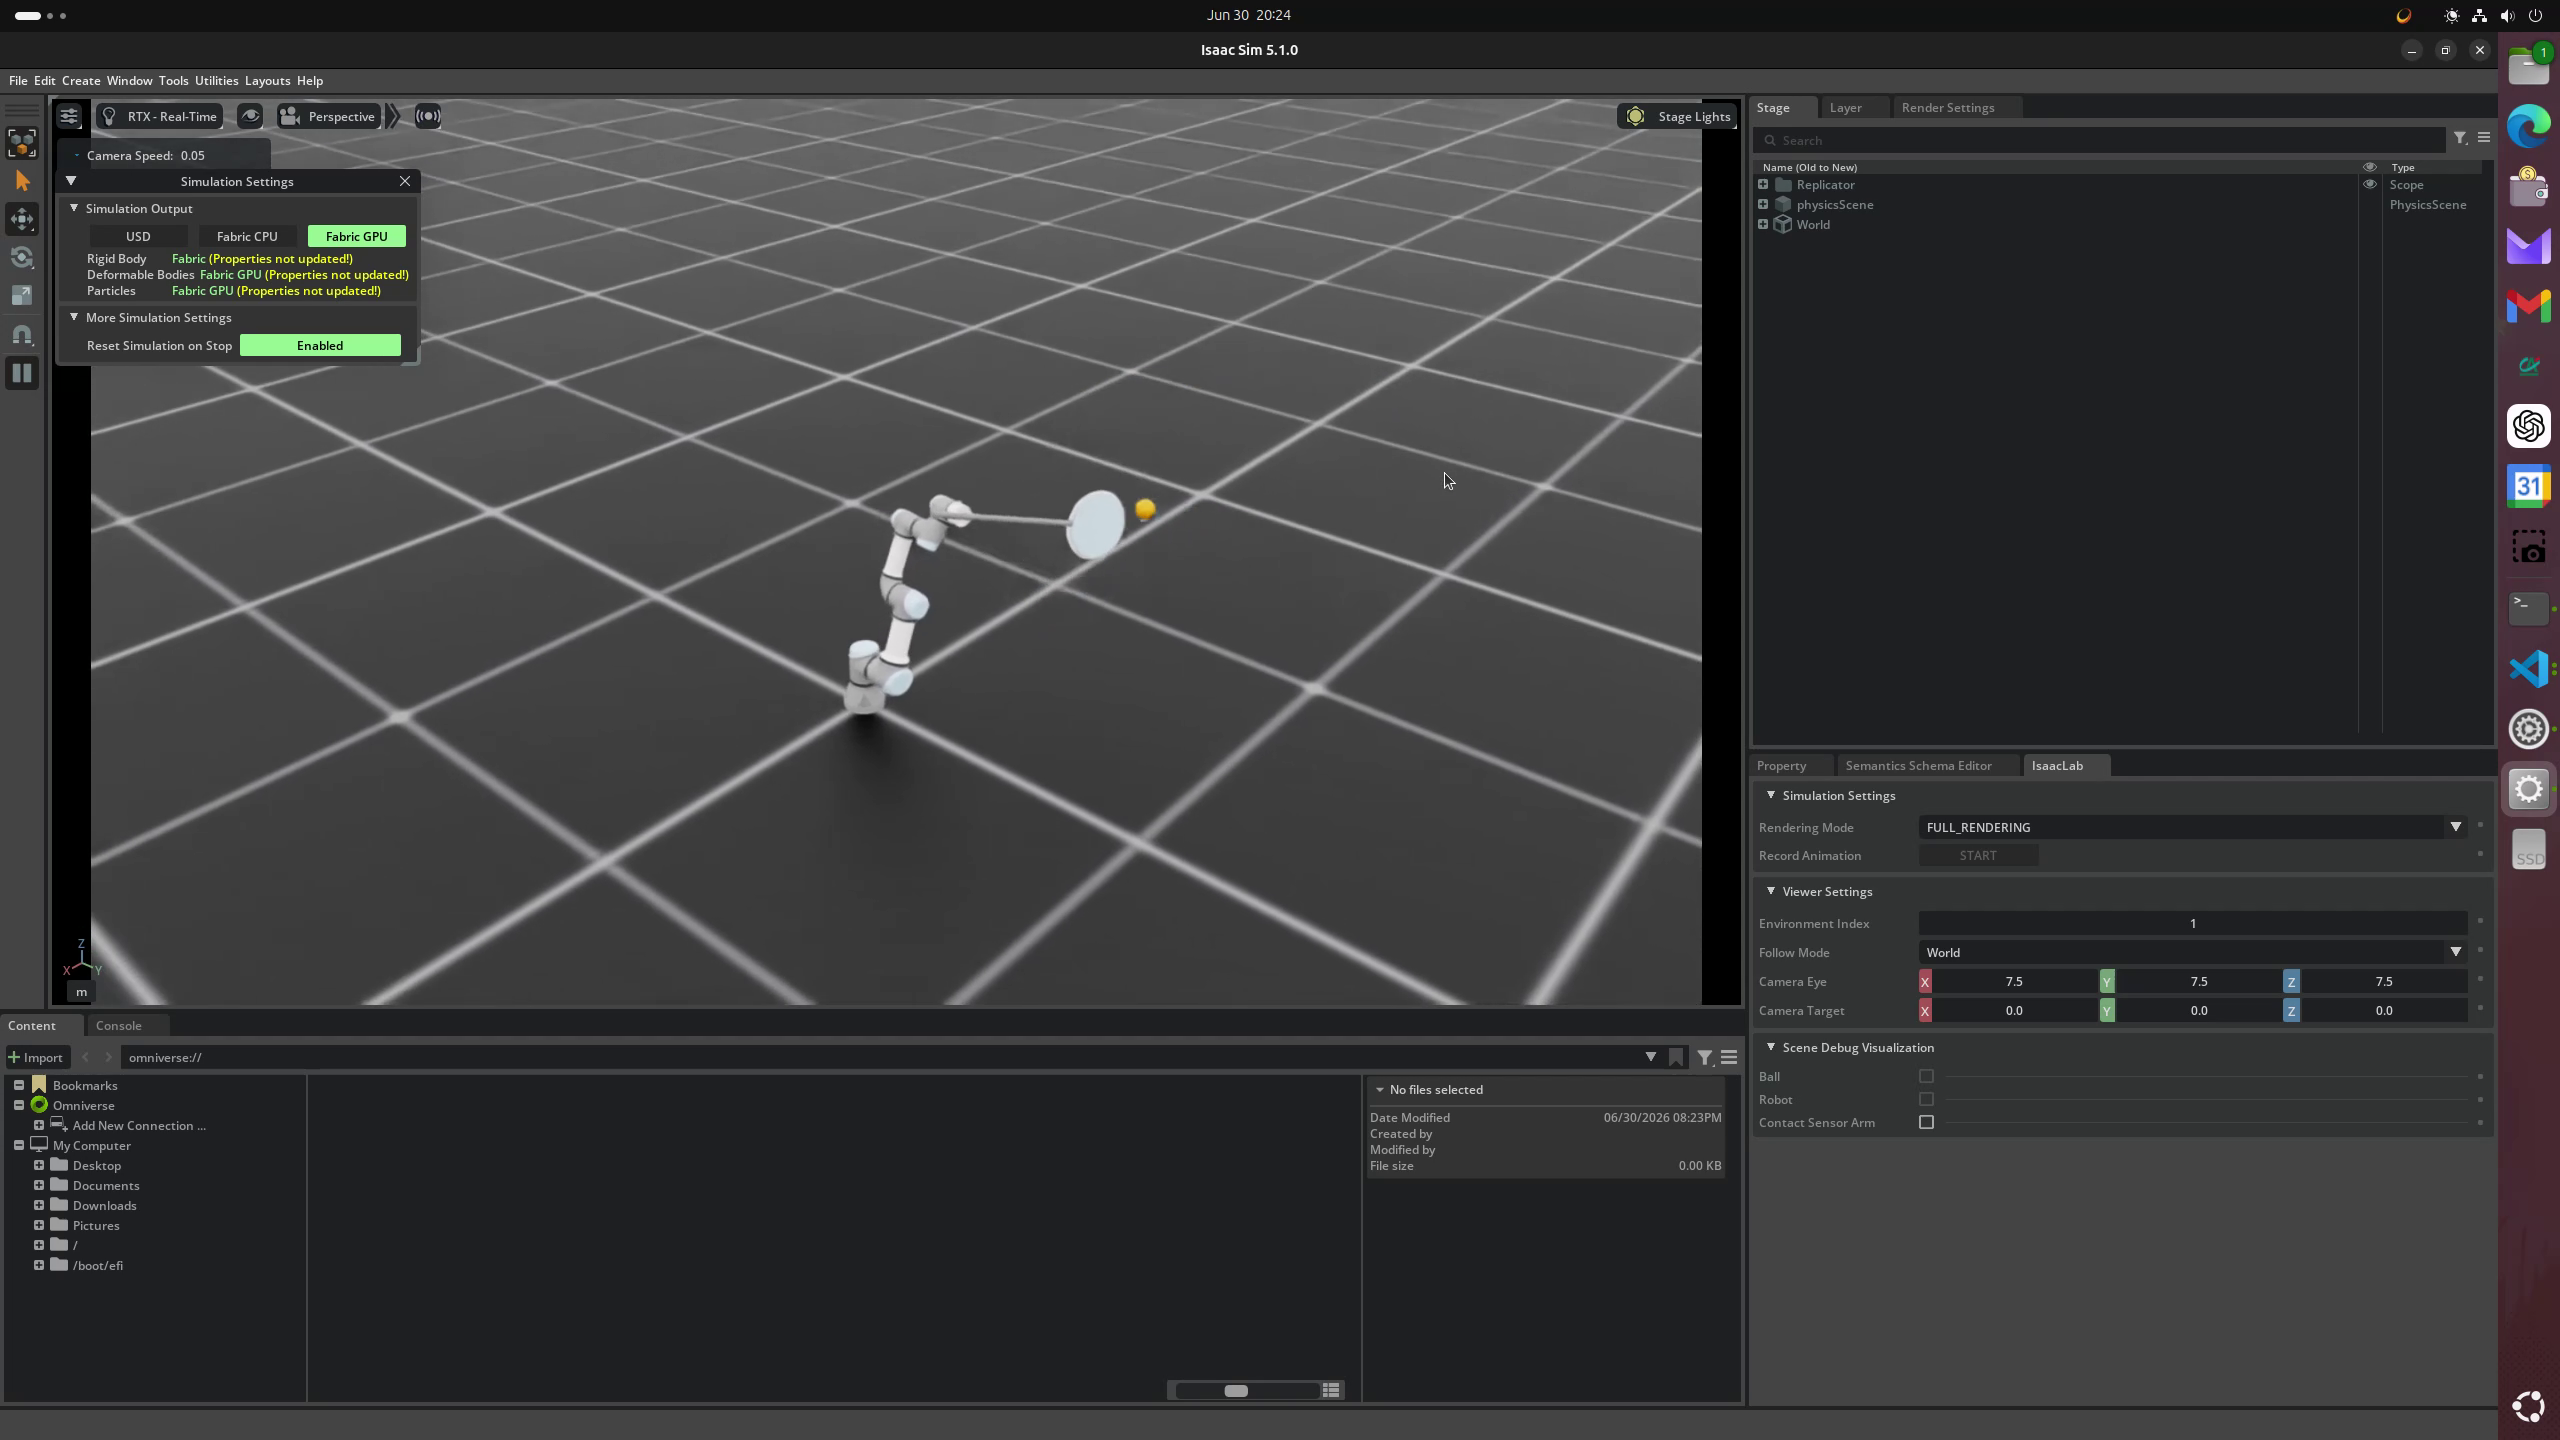
\includegraphics[width=8.10cm]{images/robot_isaac_30_juin_poster.png}}{video/Robot_isaac_30_juin.mp4}};
  \fill[deepbrown,opacity=0.62] ($(SW)+(5.16,4.18)$) circle (0.40cm);
  \draw[amber,opacity=0.92,line width=0.55pt] ($(SW)+(5.16,4.18)$) circle (0.40cm);
  \fill[amber,opacity=0.96]
    ($(SW)+(5.05,3.96)$) -- ($(SW)+(5.05,4.40)$) -- ($(SW)+(5.41,4.18)$) -- cycle;
  \node[
    anchor=center,
    text=cream,
    font=\fontsize{5.25}{5.8}\selectfont\bfseries,
    text width=7.75cm,
    align=center
  ] at ($(SW)+(5.16,1.34)$)
    {Des milliers de lancers simulés, sans risque matériel.};

  \path[trainpanel] ($(SW)+(10.04,0.92)$) rectangle ($(SW)+(15.28,7.12)$);
  \node[anchor=west,text=amber,font=\fontsize{7.0}{7.6}\selectfont\bfseries]
    at ($(SW)+(10.34,6.78)$) {Résultat obtenu};

  \path[trainmetric] ($(SW)+(10.36,5.70)$) rectangle ($(SW)+(12.62,6.42)$);
  \node[anchor=center,text=cream,font=\fontsize{11.0}{11.6}\selectfont\bfseries]
    at ($(SW)+(11.49,6.10)$) {2 h 17};
  \node[anchor=center,text=softcream,font=\fontsize{4.6}{5.0}\selectfont]
    at ($(SW)+(11.49,5.86)$) {durée entraînement};

  \path[trainmetric] ($(SW)+(12.96,5.70)$) rectangle ($(SW)+(14.96,6.42)$);
  \node[anchor=center,text=cream,font=\fontsize{11.0}{11.6}\selectfont\bfseries]
    at ($(SW)+(13.96,6.10)$) {90 \%};
  \node[anchor=center,text=softcream,font=\fontsize{4.6}{5.0}\selectfont]
    at ($(SW)+(13.96,5.86)$) {taux de succès};

  \path[trainmetric] ($(SW)+(10.36,4.56)$) rectangle ($(SW)+(12.62,5.28)$);
  \node[anchor=center,text=cream,font=\fontsize{10.0}{10.6}\selectfont\bfseries]
    at ($(SW)+(11.49,4.96)$) {2,5 ans};
  \node[anchor=center,text=softcream,font=\fontsize{4.6}{5.0}\selectfont]
    at ($(SW)+(11.49,4.72)$) {équiv. temps réel};

  \path[trainmetric] ($(SW)+(12.96,4.56)$) rectangle ($(SW)+(14.96,5.28)$);
  \node[anchor=center,text=cream,font=\fontsize{9.2}{9.8}\selectfont\bfseries]
    at ($(SW)+(13.96,4.96)$) {\(\sim 9\,600\times\)};
  \node[anchor=center,text=softcream,font=\fontsize{4.6}{5.0}\selectfont]
    at ($(SW)+(13.96,4.72)$) {accélération};

  \path[trainchip] ($(SW)+(10.36,3.46)$) rectangle ($(SW)+(14.96,4.04)$);
  \node[anchor=center,text=cream,font=\fontsize{4.95}{5.45}\selectfont\bfseries,text width=4.35cm,align=center]
    at ($(SW)+(12.66,3.75)$) {Obs. 33-D \quad Actions : 6 joints};

  \path[trainchip] ($(SW)+(10.36,2.58)$) rectangle ($(SW)+(14.96,3.16)$);
  \node[anchor=center,text=cream,font=\fontsize{5.05}{5.55}\selectfont\bfseries,text width=4.10cm,align=center]
    at ($(SW)+(12.66,2.87)$) {Pas de commande : \(1/60\) s};

  \node[
    anchor=center,
    text=cream,
    font=\fontsize{4.95}{5.45}\selectfont\bfseries,
    text width=4.42cm,
    align=center
  ] at ($(SW)+(12.66,1.76)$)
    {état balle + robot \(\rightarrow\) \textcolor{amber}{PPO} \(\rightarrow\) cibles articulaires};

  \node[
    anchor=center,
    text=softcream,
    font=\fontsize{4.55}{4.95}\selectfont,
    text width=4.35cm,
    align=center
  ] at ($(SW)+(12.66,1.18)$)
    {Politique exportée ensuite pour l'intégration ROS 2 / UR3e.};
  \node[
    anchor=south east,
    text=softcream,
    font=\fontsize{4.7}{5.0}\selectfont,
    opacity=0.75
  ] at ($(SW)+(15.50,0.40)$) {11 / 13};
\end{tikzpicture}

\newpage

\begin{tikzpicture}[remember picture,overlay]
  \path (current page.south west) coordinate (SW);
  \path (current page.north east) coordinate (NE);

  \shade[left color=deepbrown,right color=redbrown] (SW) rectangle (NE);
  \fill[rust,opacity=0.35]
    (SW) -- ($(SW)+(5.7,0)$) -- ($(NE)+(-5.0,0)$) -- ($(NE)+(-9.4,0)$) -- cycle;
  \fill[orangehot,opacity=0.18]
    ($(SW)+(0,0)$) -- ($(SW)+(2.7,0)$) -- ($(NE)+(-7.2,0)$) -- ($(NE)+(-10.6,0)$) -- cycle;
  \fill[deepbrown,opacity=0.28] (SW) rectangle (NE);

  \node[
    anchor=west,
    text=cream,
    font=\fontsize{20}{22}\selectfont\bfseries
  ] at ($(SW)+(0.72,8.20)$) {Nœuds ROS 2 : de la balle au robot};
  \draw[orangehot,line width=0.85pt] ($(SW)+(0.74,7.88)$) -- ($(SW)+(8.55,7.88)$);
  \draw[amber,line width=0.40pt,opacity=0.75] ($(SW)+(0.74,7.75)$) -- ($(SW)+(4.60,7.75)$);

  \tikzset{
    rospanel/.style={
      fill=deepbrown,
      fill opacity=0.58,
      draw=orangehot,
      draw opacity=0.84,
      line width=0.55pt,
      rounded corners=5pt
    },
    nodecard/.style={
      fill=redbrown,
      fill opacity=0.82,
      draw=amber,
      draw opacity=0.62,
      line width=0.32pt,
      rounded corners=3pt
    },
    flowarrow/.style={-{Latex[length=2.0mm]},draw=amber,opacity=0.92,line width=0.70pt},
    topictag/.style={
      fill=orangehot,
      fill opacity=0.20,
      draw=amber,
      draw opacity=0.55,
      line width=0.25pt,
      rounded corners=2.5pt
    }
  }

  % --- Left panel: live demo video ---
  \path[rospanel] ($(SW)+(0.72,1.02)$) rectangle ($(SW)+(8.62,7.12)$);
  \node[anchor=west,text=amber,font=\fontsize{7.0}{7.6}\selectfont\bfseries]
    at ($(SW)+(1.02,6.78)$) {Boucle complète sur le robot réel};
  \node[anchor=center,inner sep=0pt] at ($(SW)+(4.67,4.10)$)
    {\movie[externalviewer=false,showcontrols=true]{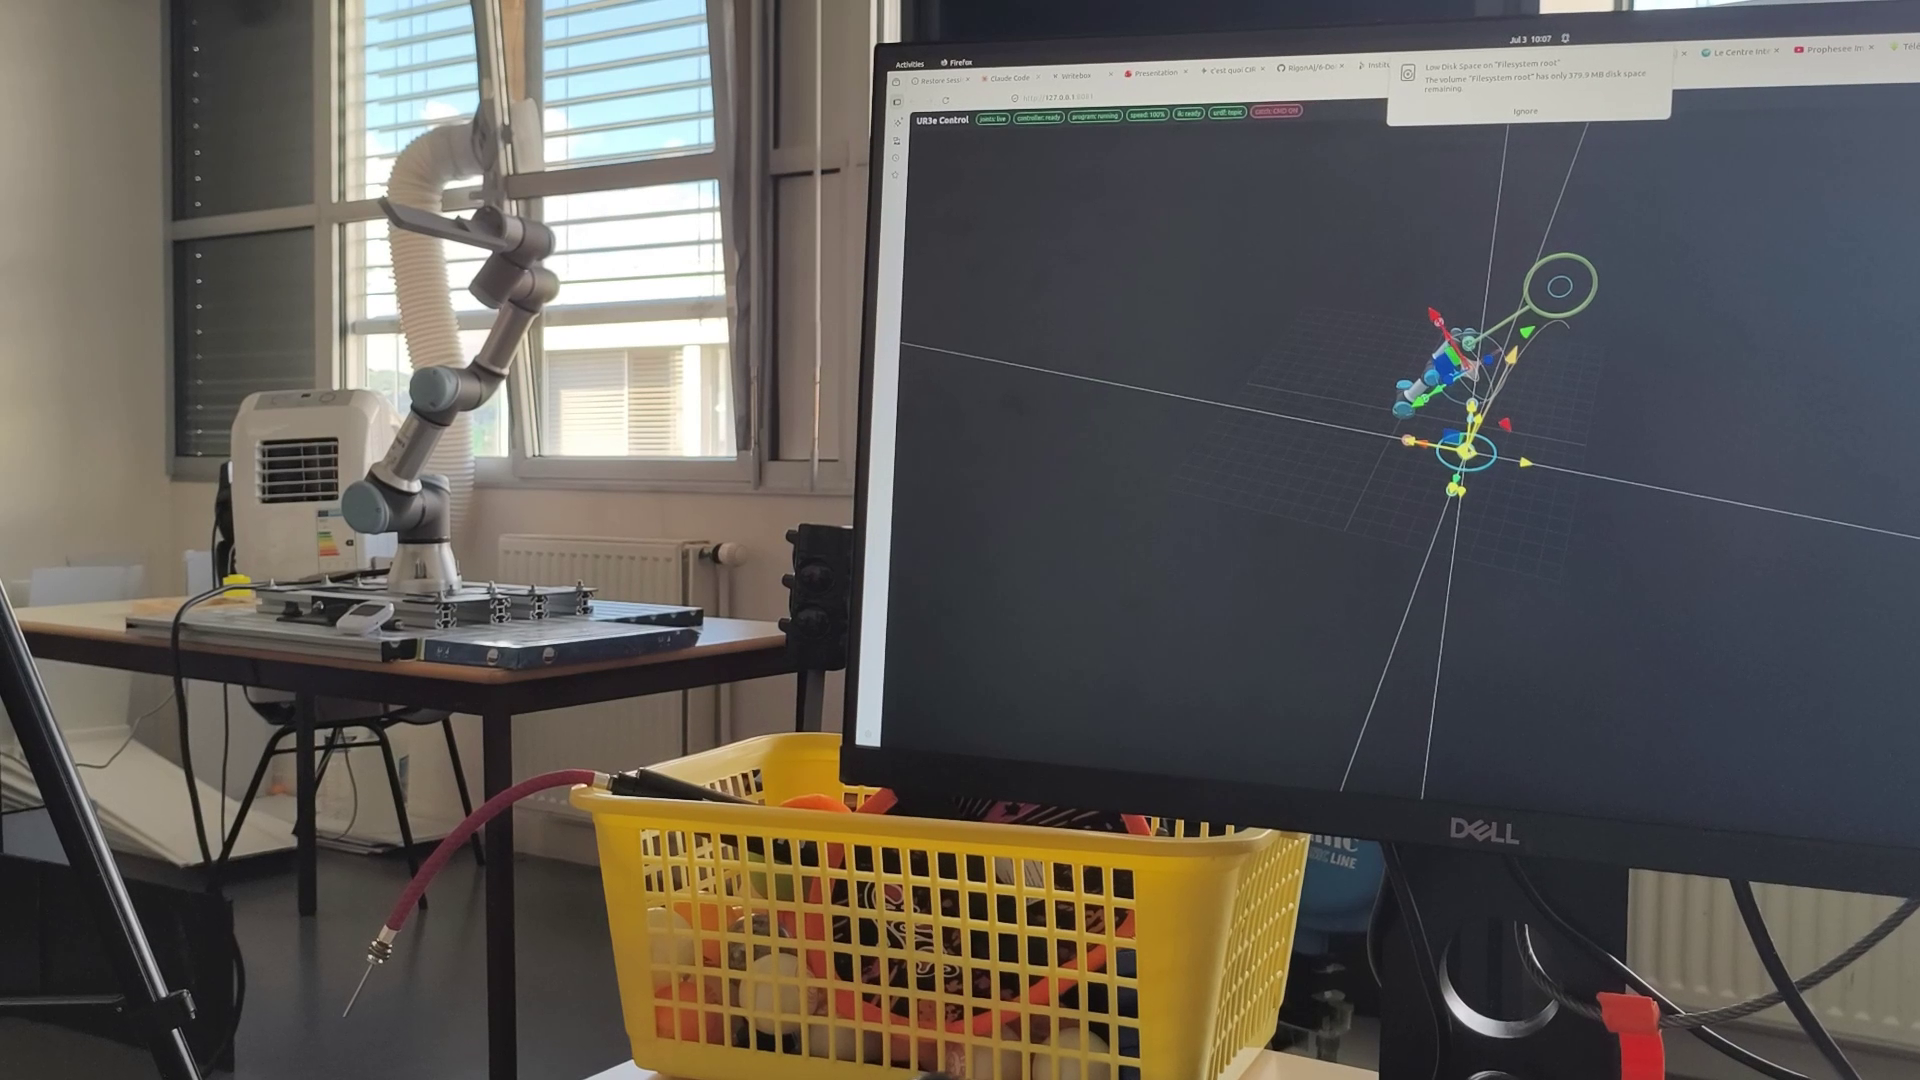
\includegraphics[width=7.05cm]{images/Test_balle_virtuelle_robot_reel_poster.png}}{video/Test_balle_virtuellle_sur_robot_reel.mp4}};
  \fill[deepbrown,opacity=0.62] ($(SW)+(4.67,4.10)$) circle (0.40cm);
  \draw[amber,opacity=0.92,line width=0.55pt] ($(SW)+(4.67,4.10)$) circle (0.40cm);
  \fill[amber,opacity=0.96]
    ($(SW)+(4.56,3.88)$) -- ($(SW)+(4.56,4.32)$) -- ($(SW)+(4.92,4.10)$) -- cycle;
  \fill[orangehot,opacity=0.15,rounded corners=3pt]
    ($(SW)+(1.10,1.30)$) rectangle ($(SW)+(8.24,1.86)$);
  \node[
    anchor=center,
    text=cream,
    font=\fontsize{5.35}{5.9}\selectfont\bfseries,
    text width=6.70cm,
    align=center
  ] at ($(SW)+(4.67,1.58)$)
    {Balle virtuelle rejouée : perception, inférence et supervision en direct.};

  % --- Right panel: three ROS 2 nodes (panel center x = 12.13) ---
  \path[rospanel] ($(SW)+(8.98,1.02)$) rectangle ($(SW)+(15.28,7.12)$);
  \node[anchor=west,text=amber,font=\fontsize{7.0}{7.6}\selectfont\bfseries]
    at ($(SW)+(9.30,6.78)$) {Trois nœuds, un même flux};

  % Node 1: perception  (card 9.26--15.00, center y = 5.98)
  \node[nodecard,minimum width=5.74cm,minimum height=1.00cm] (perc)
    at ($(SW)+(12.13,5.98)$) {};
  \fill[orangehot,rounded corners=1pt] ($(SW)+(9.40,5.60)$) rectangle ($(SW)+(9.55,6.36)$);
  \node[anchor=west,text=cream,font=\fontsize{6.4}{6.9}\selectfont\bfseries]
    at ($(SW)+(9.80,6.20)$) {Perception};
  \node[anchor=north west,text=softcream,font=\fontsize{4.7}{5.2}\selectfont,text width=4.45cm,align=left]
    at ($(SW)+(9.80,5.98)$) {Caméra événementielle $\rightarrow$ position 3D datée.};

  % Node 2: inference  (center y = 4.48)
  \node[nodecard,minimum width=5.74cm,minimum height=1.00cm] (infer)
    at ($(SW)+(12.13,4.48)$) {};
  \fill[amber,rounded corners=1pt] ($(SW)+(9.40,4.10)$) rectangle ($(SW)+(9.55,4.86)$);
  \node[anchor=west,text=cream,font=\fontsize{6.4}{6.9}\selectfont\bfseries]
    at ($(SW)+(9.80,4.70)$) {Inférence};
  \node[anchor=north west,text=softcream,font=\fontsize{4.7}{5.2}\selectfont,text width=4.45cm,align=left]
    at ($(SW)+(9.80,4.48)$) {Politique Isaac $\rightarrow$ cibles articulaires.};

  % Node 3: visualization / web ui  (center y = 2.98)
  \node[nodecard,minimum width=5.74cm,minimum height=1.00cm] (viz)
    at ($(SW)+(12.13,2.98)$) {};
  \fill[teal,rounded corners=1pt] ($(SW)+(9.40,2.60)$) rectangle ($(SW)+(9.55,3.36)$);
  \node[anchor=west,text=cream,font=\fontsize{6.4}{6.9}\selectfont\bfseries]
    at ($(SW)+(9.80,3.20)$) {Visualisation — Web UI};
  \node[anchor=north west,text=softcream,font=\fontsize{4.7}{5.2}\selectfont,text width=4.45cm,align=left]
    at ($(SW)+(9.80,2.98)$) {Supervision navigateur, vue 3D, sécurité commande.};

  % flow arrows + topic tags (arrow at x = 12.13)
  \draw[flowarrow] (perc.south) -- (infer.north);
  \node[anchor=center,text=amber,font=\fontsize{4.6}{5.0}\selectfont\ttfamily]
    at ($(SW)+(13.25,5.23)$) {/ball\_state};
  \draw[flowarrow] (infer.south) -- (viz.north);
  \node[anchor=center,text=amber,font=\fontsize{4.6}{5.0}\selectfont\ttfamily]
    at ($(SW)+(13.25,3.73)$) {/commande};

  \fill[orangehot,opacity=0.16,rounded corners=3pt]
    ($(SW)+(9.40,1.28)$) rectangle ($(SW)+(14.86,2.14)$);
  \node[
    anchor=center,
    text=cream,
    font=\fontsize{5.0}{5.6}\selectfont\bfseries,
    text width=5.05cm,
    align=center
  ] at ($(SW)+(12.13,1.71)$)
    {La Web UI observe la balle et le robot, et garde la main sur les commandes.};
  \node[
    anchor=south east,
    text=softcream,
    font=\fontsize{4.7}{5.0}\selectfont,
    opacity=0.75
  ] at ($(SW)+(15.50,0.40)$) {12 / 13};
\end{tikzpicture}

\newpage

\begin{tikzpicture}[remember picture,overlay]
  \path (current page.south west) coordinate (SW);
  \path (current page.north east) coordinate (NE);

  \shade[left color=deepbrown,right color=redbrown] (SW) rectangle (NE);
  \fill[rust,opacity=0.35]
    (SW) -- ($(SW)+(5.7,0)$) -- ($(NE)+(-5.0,0)$) -- ($(NE)+(-9.4,0)$) -- cycle;
  \fill[orangehot,opacity=0.18]
    ($(SW)+(0,0)$) -- ($(SW)+(2.7,0)$) -- ($(NE)+(-7.2,0)$) -- ($(NE)+(-10.6,0)$) -- cycle;
  \fill[deepbrown,opacity=0.28] (SW) rectangle (NE);

  \node[
    anchor=west,
    text=cream,
    font=\fontsize{20}{22}\selectfont\bfseries
  ] at ($(SW)+(0.72,8.20)$) {Ce qu'il reste à faire};
  \draw[orangehot,line width=0.85pt] ($(SW)+(0.74,7.88)$) -- ($(SW)+(5.35,7.88)$);
  \draw[amber,line width=0.40pt,opacity=0.75] ($(SW)+(0.74,7.75)$) -- ($(SW)+(2.95,7.75)$);

  \tikzset{
    todopanel/.style={
      fill=deepbrown,
      fill opacity=0.58,
      draw=orangehot,
      draw opacity=0.84,
      line width=0.55pt,
      rounded corners=5pt
    },
    checkbox/.style={
      draw=amber,
      line width=0.5pt,
      rounded corners=1pt,
      minimum size=0.30cm,
      inner sep=0pt,
      fill=orangehot,
      fill opacity=0.14
    }
  }

  % --- Left panel: montage & calibration (hardware) ---
  \path[todopanel] ($(SW)+(0.72,1.18)$) rectangle ($(SW)+(7.70,7.12)$);
  \node[anchor=west,text=amber,font=\fontsize{7.0}{7.6}\selectfont\bfseries]
    at ($(SW)+(1.02,6.78)$) {Montage \& calibration};

  \node[checkbox] at ($(SW)+(1.24,5.85)$) {};
  \node[anchor=west,text=cream,font=\fontsize{6.4}{6.9}\selectfont\bfseries]
    at ($(SW)+(1.58,5.99)$) {Calibration extrinsèque};
  \node[anchor=north west,text=softcream,font=\fontsize{4.8}{5.3}\selectfont,text width=5.60cm,align=left]
    at ($(SW)+(1.58,5.77)$) {Main-œil base $\leftrightarrow$ caméra : pas encore réalisée.};

  \node[checkbox] at ($(SW)+(1.24,4.25)$) {};
  \node[anchor=west,text=cream,font=\fontsize{6.4}{6.9}\selectfont\bfseries]
    at ($(SW)+(1.58,4.39)$) {Support du filet imprimé};
  \node[anchor=north west,text=softcream,font=\fontsize{4.8}{5.3}\selectfont,text width=5.60cm,align=left]
    at ($(SW)+(1.58,4.17)$) {Pièce 3D qui maintient le filet à papillon sur le \mbox{poignet}.};

  \node[checkbox] at ($(SW)+(1.24,2.65)$) {};
  \node[anchor=west,text=cream,font=\fontsize{6.4}{6.9}\selectfont\bfseries]
    at ($(SW)+(1.58,2.79)$) {Repères TF publiés};
  \node[anchor=north west,text=softcream,font=\fontsize{4.8}{5.3}\selectfont,text width=5.60cm,align=left]
    at ($(SW)+(1.58,2.57)$) {base $\rightarrow$ caméra et poignet $\rightarrow$ centre du filet.};

  % --- Right panel: intégration & validation (chaîne complète) ---
  \path[todopanel] ($(SW)+(8.30,1.18)$) rectangle ($(SW)+(15.28,7.12)$);
  \node[anchor=west,text=amber,font=\fontsize{7.0}{7.6}\selectfont\bfseries]
    at ($(SW)+(8.60,6.78)$) {Intégration \& validation};

  \node[checkbox] at ($(SW)+(8.82,5.85)$) {};
  \node[anchor=west,text=cream,font=\fontsize{6.4}{6.9}\selectfont\bfseries]
    at ($(SW)+(9.16,5.99)$) {Test de la chaîne complète};
  \node[anchor=north west,text=softcream,font=\fontsize{4.8}{5.3}\selectfont,text width=5.65cm,align=left]
    at ($(SW)+(9.16,5.77)$) {Caméra événementielle + inférence + robot réel, bout en bout.};

  \node[checkbox] at ($(SW)+(8.82,4.25)$) {};
  \node[anchor=west,text=cream,font=\fontsize{6.4}{6.9}\selectfont\bfseries]
    at ($(SW)+(9.16,4.39)$) {Réactivité \& latence};
  \node[anchor=north west,text=softcream,font=\fontsize{4.8}{5.3}\selectfont,text width=5.65cm,align=left]
    at ($(SW)+(9.16,4.17)$) {Accélérer le robot, encore lent ; mesurer la latence bout en bout.};

  % --- bottom objective banner (full width) ---
  \fill[orangehot,opacity=0.18,rounded corners=3pt]
    ($(SW)+(0.72,0.34)$) rectangle ($(SW)+(15.28,0.98)$);
  \node[
    anchor=center,
    text=cream,
    font=\fontsize{5.8}{6.3}\selectfont\bfseries,
    text width=13.8cm,
    align=center
  ] at ($(SW)+(8.00,0.66)$)
    {Objectif : une première interception réelle, de la caméra au filet.};
  \node[
    anchor=south east,
    text=softcream,
    font=\fontsize{4.7}{5.0}\selectfont,
    opacity=0.75
  ] at ($(SW)+(15.50,0.40)$) {13 / 13};
\end{tikzpicture}

\end{document}
